\documentclass[twoside]{book}

% Packages required by doxygen
\usepackage{fixltx2e}
\usepackage{calc}
\usepackage{doxygen}
\usepackage[export]{adjustbox} % also loads graphicx
\usepackage{graphicx}
\usepackage[utf8]{inputenc}
\usepackage{makeidx}
\usepackage{multicol}
\usepackage{multirow}
\PassOptionsToPackage{warn}{textcomp}
\usepackage{textcomp}
\usepackage[nointegrals]{wasysym}
\usepackage[table]{xcolor}

% Font selection
\usepackage[T1]{fontenc}
\usepackage[scaled=.90]{helvet}
\usepackage{courier}
\usepackage{amssymb}
\usepackage{sectsty}
\renewcommand{\familydefault}{\sfdefault}
\allsectionsfont{%
  \fontseries{bc}\selectfont%
  \color{darkgray}%
}
\renewcommand{\DoxyLabelFont}{%
  \fontseries{bc}\selectfont%
  \color{darkgray}%
}
\newcommand{\+}{\discretionary{\mbox{\scriptsize$\hookleftarrow$}}{}{}}

% Page & text layout
\usepackage{geometry}
\geometry{%
  a4paper,%
  top=2.5cm,%
  bottom=2.5cm,%
  left=2.5cm,%
  right=2.5cm%
}
\tolerance=750
\hfuzz=15pt
\hbadness=750
\setlength{\emergencystretch}{15pt}
\setlength{\parindent}{0cm}
\setlength{\parskip}{3ex plus 2ex minus 2ex}
\makeatletter
\renewcommand{\paragraph}{%
  \@startsection{paragraph}{4}{0ex}{-1.0ex}{1.0ex}{%
    \normalfont\normalsize\bfseries\SS@parafont%
  }%
}
\renewcommand{\subparagraph}{%
  \@startsection{subparagraph}{5}{0ex}{-1.0ex}{1.0ex}{%
    \normalfont\normalsize\bfseries\SS@subparafont%
  }%
}
\makeatother

% Headers & footers
\usepackage{fancyhdr}
\pagestyle{fancyplain}
\fancyhead[LE]{\fancyplain{}{\bfseries\thepage}}
\fancyhead[CE]{\fancyplain{}{}}
\fancyhead[RE]{\fancyplain{}{\bfseries\leftmark}}
\fancyhead[LO]{\fancyplain{}{\bfseries\rightmark}}
\fancyhead[CO]{\fancyplain{}{}}
\fancyhead[RO]{\fancyplain{}{\bfseries\thepage}}
\fancyfoot[LE]{\fancyplain{}{}}
\fancyfoot[CE]{\fancyplain{}{}}
\fancyfoot[RE]{\fancyplain{}{\bfseries\scriptsize Generated by Doxygen }}
\fancyfoot[LO]{\fancyplain{}{\bfseries\scriptsize Generated by Doxygen }}
\fancyfoot[CO]{\fancyplain{}{}}
\fancyfoot[RO]{\fancyplain{}{}}
\renewcommand{\footrulewidth}{0.4pt}
\renewcommand{\chaptermark}[1]{%
  \markboth{#1}{}%
}
\renewcommand{\sectionmark}[1]{%
  \markright{\thesection\ #1}%
}

% Indices & bibliography
\usepackage{natbib}
\usepackage[titles]{tocloft}
\setcounter{tocdepth}{3}
\setcounter{secnumdepth}{5}
\makeindex

% Hyperlinks (required, but should be loaded last)
\usepackage{ifpdf}
\ifpdf
  \usepackage[pdftex,pagebackref=true]{hyperref}
\else
  \usepackage[ps2pdf,pagebackref=true]{hyperref}
\fi
\hypersetup{%
  colorlinks=true,%
  linkcolor=blue,%
  citecolor=blue,%
  unicode%
}

% Custom commands
\newcommand{\clearemptydoublepage}{%
  \newpage{\pagestyle{empty}\cleardoublepage}%
}

\usepackage{caption}
\captionsetup{labelsep=space,justification=centering,font={bf},singlelinecheck=off,skip=4pt,position=top}

%===== C O N T E N T S =====

\begin{document}

% Titlepage & ToC
\hypersetup{pageanchor=false,
             bookmarksnumbered=true,
             pdfencoding=unicode
            }
\pagenumbering{alph}
\begin{titlepage}
\vspace*{7cm}
\begin{center}%
{\Large Arbutus }\\
\vspace*{1cm}
{\large Generated by Doxygen 1.8.13}\\
\end{center}
\end{titlepage}
\clearemptydoublepage
\pagenumbering{roman}
\tableofcontents
\clearemptydoublepage
\pagenumbering{arabic}
\hypersetup{pageanchor=true}

%--- Begin generated contents ---
\chapter{Hierarchical Index}
\section{Class Hierarchy}
This inheritance list is sorted roughly, but not completely, alphabetically\+:\begin{DoxyCompactList}
\item \contentsline{section}{Element}{\pageref{class_element}}{}
\begin{DoxyCompactList}
\item \contentsline{section}{Button}{\pageref{class_button}}{}
\begin{DoxyCompactList}
\item \contentsline{section}{Slider}{\pageref{class_slider}}{}
\begin{DoxyCompactList}
\item \contentsline{section}{Vertical\+Slider}{\pageref{class_vertical_slider}}{}
\end{DoxyCompactList}
\end{DoxyCompactList}
\item \contentsline{section}{Splitter}{\pageref{class_splitter}}{}
\item \contentsline{section}{Viewport}{\pageref{class_viewport}}{}
\end{DoxyCompactList}
\item \contentsline{section}{G\+UI}{\pageref{class_g_u_i}}{}
\item \contentsline{section}{G\+U\+I\+Style}{\pageref{class_g_u_i_style}}{}
\item of\+Base\+App\begin{DoxyCompactList}
\item \contentsline{section}{of\+App}{\pageref{classof_app}}{}
\end{DoxyCompactList}
\item \contentsline{section}{Splitter\+Child}{\pageref{struct_splitter_child}}{}
\item \contentsline{section}{Trigger\+Visual\+Action}{\pageref{class_trigger_visual_action}}{}
\end{DoxyCompactList}

\chapter{Class Index}
\section{Class List}
Here are the classes, structs, unions and interfaces with brief descriptions\+:\begin{DoxyCompactList}
\item\contentsline{section}{\hyperlink{class_button}{Button} }{\pageref{class_button}}{}
\item\contentsline{section}{\hyperlink{class_element}{Element} }{\pageref{class_element}}{}
\item\contentsline{section}{\hyperlink{class_g_u_i}{G\+UI} }{\pageref{class_g_u_i}}{}
\item\contentsline{section}{\hyperlink{class_g_u_i_style}{G\+U\+I\+Style} }{\pageref{class_g_u_i_style}}{}
\item\contentsline{section}{\hyperlink{classof_app}{of\+App} }{\pageref{classof_app}}{}
\item\contentsline{section}{\hyperlink{class_slider}{Slider} }{\pageref{class_slider}}{}
\item\contentsline{section}{\hyperlink{class_splitter}{Splitter} }{\pageref{class_splitter}}{}
\item\contentsline{section}{\hyperlink{struct_splitter_child}{Splitter\+Child} }{\pageref{struct_splitter_child}}{}
\item\contentsline{section}{\hyperlink{class_trigger_visual_action}{Trigger\+Visual\+Action} }{\pageref{class_trigger_visual_action}}{}
\item\contentsline{section}{\hyperlink{class_vertical_slider}{Vertical\+Slider} }{\pageref{class_vertical_slider}}{}
\item\contentsline{section}{\hyperlink{class_viewport}{Viewport} }{\pageref{class_viewport}}{}
\end{DoxyCompactList}

\chapter{Class Documentation}
\hypertarget{class_button}{}\section{Button Class Reference}
\label{class_button}\index{Button@{Button}}


{\ttfamily \#include $<$Button.\+hpp$>$}

Inheritance diagram for Button\+:\begin{figure}[H]
\begin{center}
\leavevmode
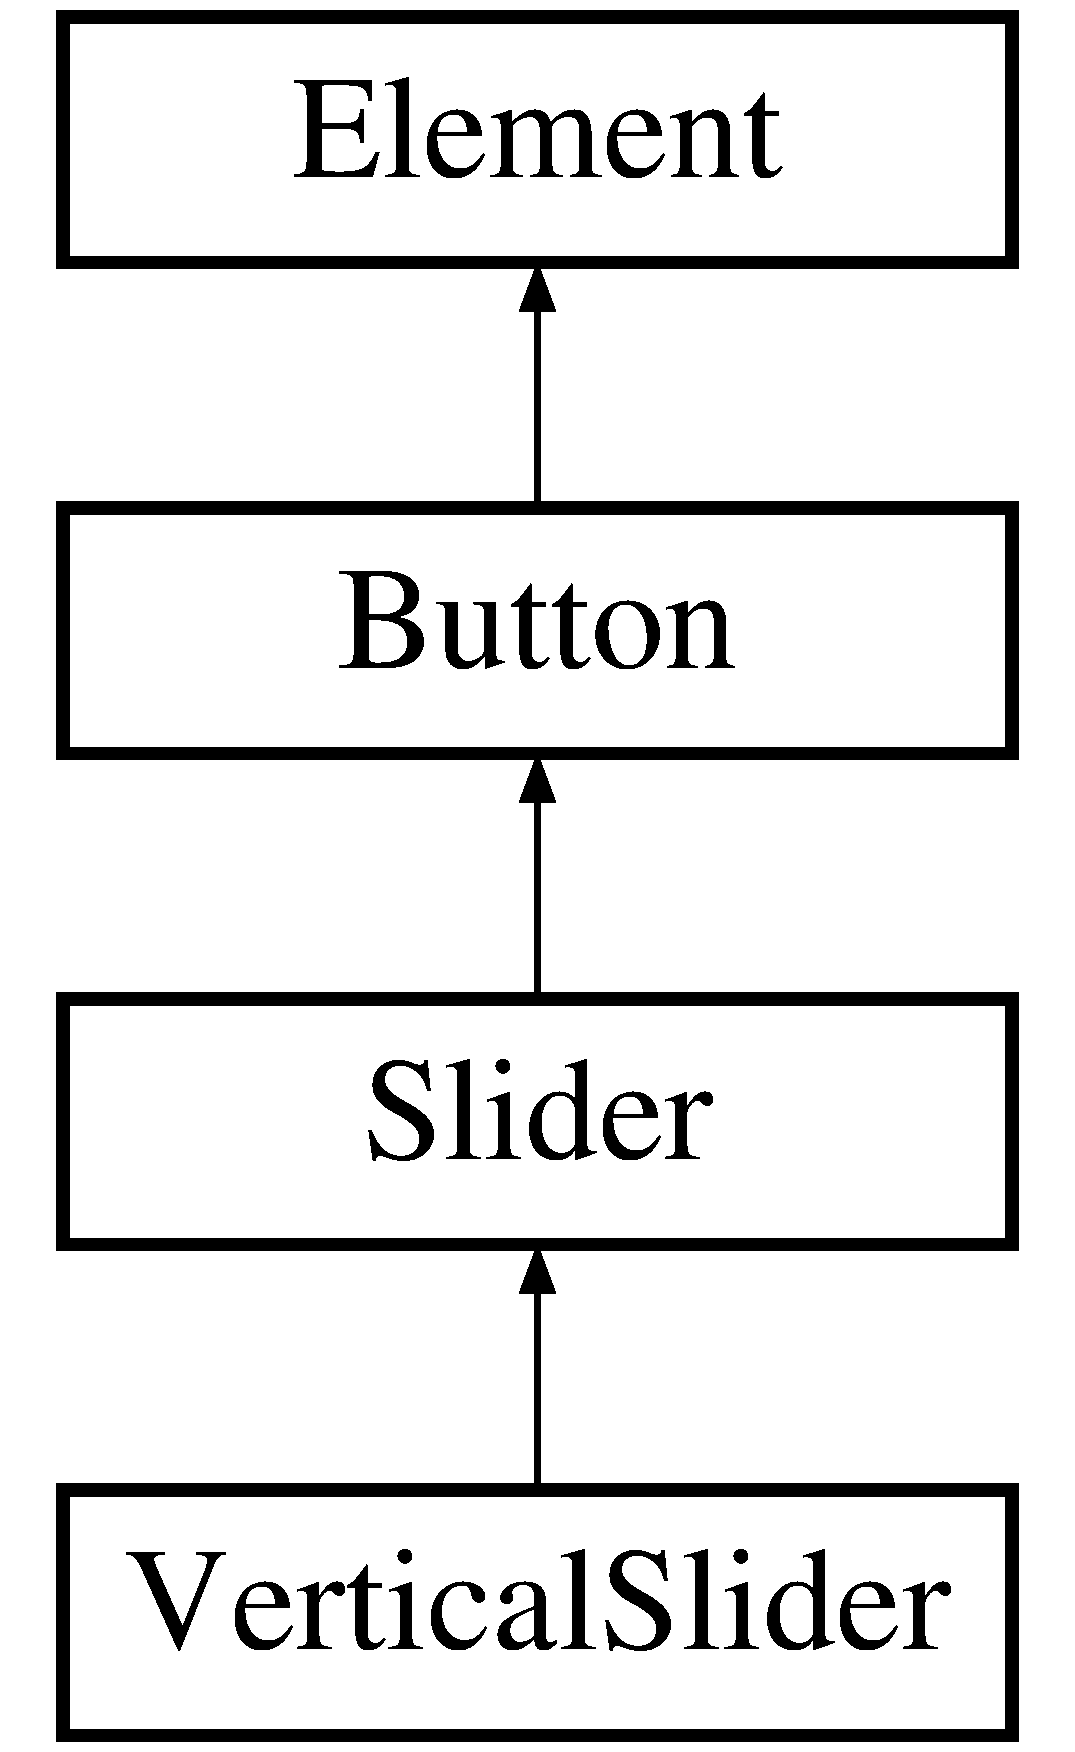
\includegraphics[height=4.000000cm]{class_button}
\end{center}
\end{figure}
\subsection*{Public Member Functions}
\begin{DoxyCompactItemize}
\item 
\hyperlink{class_button_a3b36df1ae23c58aedb9e15a713159459}{Button} ()
\item 
\hyperlink{class_button_a2a001eb9c3cc8ae54768a850dd345002}{$\sim$\+Button} ()
\item 
virtual void \hyperlink{class_button_ad8e030c1c8846d43f3126047d4a3667f}{update} ()
\item 
virtual void \hyperlink{class_button_a3a6ae66dc1ebc663fc12f19ce5cb6840}{draw} (N\+V\+Gcontext $\ast$vg)
\item 
virtual void \hyperlink{class_button_a6e7c3b800fae0b1e7765ccdafc88c28e}{set} (json config)
\item 
void \hyperlink{class_button_a0e4d6981ae08afd292ffa9a9f01939df}{set\+On\+Click} (std\+::function$<$ void(\hyperlink{class_button}{Button} $\ast$button)$>$ \+\_\+on\+Click)
\item 
virtual string \hyperlink{class_button_ad22978c530f78e58cb213436b24b37c0}{get\+Class} ()
\end{DoxyCompactItemize}
\subsection*{Protected Attributes}
\begin{DoxyCompactItemize}
\item 
\mbox{\Hypertarget{class_button_af6ed106421f242c44f954440e419cf18}\label{class_button_af6ed106421f242c44f954440e419cf18}} 
Boolean {\bfseries pushed}
\item 
\mbox{\Hypertarget{class_button_a265d7cb5d80829f7195344f773069c0b}\label{class_button_a265d7cb5d80829f7195344f773069c0b}} 
string {\bfseries caption}
\item 
\mbox{\Hypertarget{class_button_a37251a2866eec58f8a56772a327bd984}\label{class_button_a37251a2866eec58f8a56772a327bd984}} 
std\+::function$<$ void(\hyperlink{class_button}{Button} $\ast$button)$>$ {\bfseries on\+Click} = N\+U\+LL
\end{DoxyCompactItemize}
\subsection*{Additional Inherited Members}


\subsection{Detailed Description}
Implements a simple button  The button have a caption and an associated lambda to be executed whenever it\textquotesingle{}s pushed. 

\subsection{Constructor \& Destructor Documentation}
\mbox{\Hypertarget{class_button_a3b36df1ae23c58aedb9e15a713159459}\label{class_button_a3b36df1ae23c58aedb9e15a713159459}} 
\index{Button@{Button}!Button@{Button}}
\index{Button@{Button}!Button@{Button}}
\subsubsection{\texorpdfstring{Button()}{Button()}}
{\footnotesize\ttfamily Button\+::\+Button (\begin{DoxyParamCaption}{ }\end{DoxyParamCaption})}

... \mbox{\Hypertarget{class_button_a2a001eb9c3cc8ae54768a850dd345002}\label{class_button_a2a001eb9c3cc8ae54768a850dd345002}} 
\index{Button@{Button}!````~Button@{$\sim$\+Button}}
\index{````~Button@{$\sim$\+Button}!Button@{Button}}
\subsubsection{\texorpdfstring{$\sim$\+Button()}{~Button()}}
{\footnotesize\ttfamily Button\+::$\sim$\+Button (\begin{DoxyParamCaption}{ }\end{DoxyParamCaption})}

... 

\subsection{Member Function Documentation}
\mbox{\Hypertarget{class_button_a3a6ae66dc1ebc663fc12f19ce5cb6840}\label{class_button_a3a6ae66dc1ebc663fc12f19ce5cb6840}} 
\index{Button@{Button}!draw@{draw}}
\index{draw@{draw}!Button@{Button}}
\subsubsection{\texorpdfstring{draw()}{draw()}}
{\footnotesize\ttfamily void Button\+::draw (\begin{DoxyParamCaption}\item[{N\+V\+Gcontext $\ast$}]{vg }\end{DoxyParamCaption})\hspace{0.3cm}{\ttfamily [virtual]}}

... 

Reimplemented from \hyperlink{class_element_a37c9abed5bec87d9ce0a5e74fb872f34}{Element}.



Reimplemented in \hyperlink{class_slider_a1db885ef790b09aee48c7344181c5424}{Slider}, and \hyperlink{class_vertical_slider_a6a5ab2800438817cc5a97c475fad9f2f}{Vertical\+Slider}.

\mbox{\Hypertarget{class_button_ad22978c530f78e58cb213436b24b37c0}\label{class_button_ad22978c530f78e58cb213436b24b37c0}} 
\index{Button@{Button}!get\+Class@{get\+Class}}
\index{get\+Class@{get\+Class}!Button@{Button}}
\subsubsection{\texorpdfstring{get\+Class()}{getClass()}}
{\footnotesize\ttfamily virtual string Button\+::get\+Class (\begin{DoxyParamCaption}{ }\end{DoxyParamCaption})\hspace{0.3cm}{\ttfamily [inline]}, {\ttfamily [virtual]}}

... 

Reimplemented from \hyperlink{class_element}{Element}.



Reimplemented in \hyperlink{class_slider_a0e917883961af99856847e571a461689}{Slider}, and \hyperlink{class_vertical_slider_a5e13fb542bdca4cca91f96ca15b28fad}{Vertical\+Slider}.

\mbox{\Hypertarget{class_button_a6e7c3b800fae0b1e7765ccdafc88c28e}\label{class_button_a6e7c3b800fae0b1e7765ccdafc88c28e}} 
\index{Button@{Button}!set@{set}}
\index{set@{set}!Button@{Button}}
\subsubsection{\texorpdfstring{set()}{set()}}
{\footnotesize\ttfamily void Button\+::set (\begin{DoxyParamCaption}\item[{json}]{config }\end{DoxyParamCaption})\hspace{0.3cm}{\ttfamily [virtual]}}

... 

Reimplemented from \hyperlink{class_element_af89dcf0a470753cf1fecd8556a802c63}{Element}.



Reimplemented in \hyperlink{class_slider_a834dbe16812e7bd4f0472882b0619ea9}{Slider}, and \hyperlink{class_vertical_slider_a35b7771bd63647aa288f16719611b567}{Vertical\+Slider}.

\mbox{\Hypertarget{class_button_a0e4d6981ae08afd292ffa9a9f01939df}\label{class_button_a0e4d6981ae08afd292ffa9a9f01939df}} 
\index{Button@{Button}!set\+On\+Click@{set\+On\+Click}}
\index{set\+On\+Click@{set\+On\+Click}!Button@{Button}}
\subsubsection{\texorpdfstring{set\+On\+Click()}{setOnClick()}}
{\footnotesize\ttfamily void Button\+::set\+On\+Click (\begin{DoxyParamCaption}\item[{std\+::function$<$ void(\hyperlink{class_button}{Button} $\ast$button)$>$}]{\+\_\+on\+Click }\end{DoxyParamCaption})}

... \mbox{\Hypertarget{class_button_ad8e030c1c8846d43f3126047d4a3667f}\label{class_button_ad8e030c1c8846d43f3126047d4a3667f}} 
\index{Button@{Button}!update@{update}}
\index{update@{update}!Button@{Button}}
\subsubsection{\texorpdfstring{update()}{update()}}
{\footnotesize\ttfamily void Button\+::update (\begin{DoxyParamCaption}{ }\end{DoxyParamCaption})\hspace{0.3cm}{\ttfamily [virtual]}}

... 

Reimplemented from \hyperlink{class_element_a35de04f6ab79440bb44083d8b300b87d}{Element}.



Reimplemented in \hyperlink{class_slider_a8bcc94829fa9c1546097da4e797665cb}{Slider}, and \hyperlink{class_vertical_slider_ae868b87e37fbdac6e4906ac6b9ad465d}{Vertical\+Slider}.



The documentation for this class was generated from the following files\+:\begin{DoxyCompactItemize}
\item 
src/\+G\+U\+I/Button.\+hpp\item 
src/\+G\+U\+I/Button.\+cpp\end{DoxyCompactItemize}

\hypertarget{class_element}{}\section{Element Class Reference}
\label{class_element}\index{Element@{Element}}


{\ttfamily \#include $<$Element.\+hpp$>$}

Inheritance diagram for Element\+:\begin{figure}[H]
\begin{center}
\leavevmode
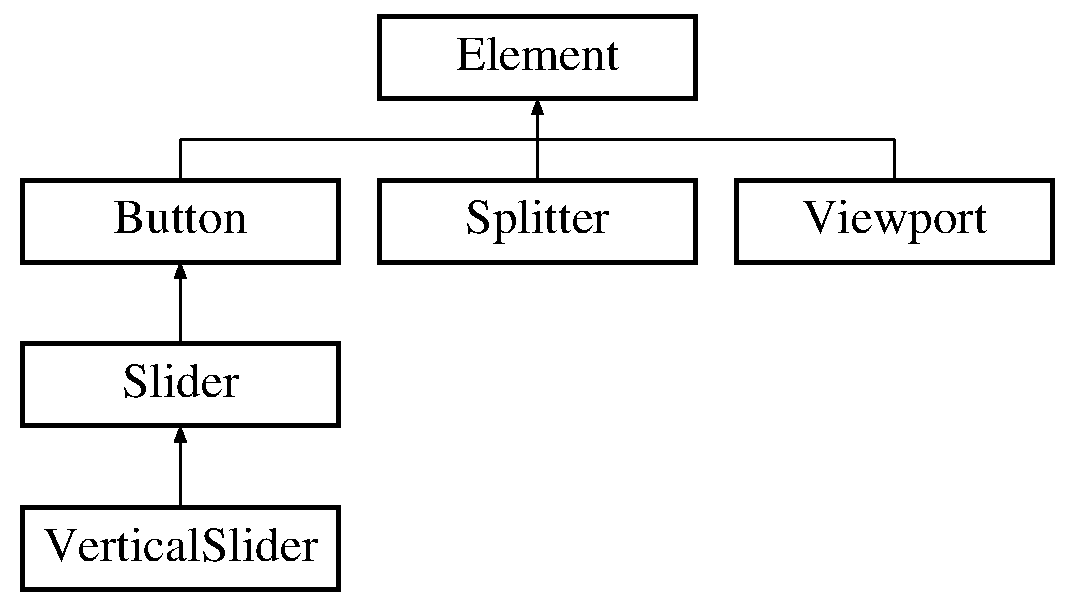
\includegraphics[height=4.000000cm]{class_element}
\end{center}
\end{figure}
\subsection*{Public Member Functions}
\begin{DoxyCompactItemize}
\item 
\hyperlink{class_element_ab0d0e20be9a36ae676202db753faeec9}{Element} ()
\item 
\hyperlink{class_element_a13d54ba9c08b6bec651402f1c2bb002c}{$\sim$\+Element} ()
\item 
\mbox{\Hypertarget{class_element_a41f73faaa553135f856f86919ca076bc}\label{class_element_a41f73faaa553135f856f86919ca076bc}} 
virtual string {\bfseries get\+Class} ()
\item 
virtual void \hyperlink{class_element_a35de04f6ab79440bb44083d8b300b87d}{update} ()
\item 
virtual void \hyperlink{class_element_a37c9abed5bec87d9ce0a5e74fb872f34}{draw} (N\+V\+Gcontext $\ast$vg)
\item 
void \hyperlink{class_element_a8b134081551b47cd3dabdd34355fa222}{finish\+Draw} (N\+V\+Gcontext $\ast$vg)
\item 
virtual void \hyperlink{class_element_af89dcf0a470753cf1fecd8556a802c63}{set} (json config)
\item 
std\+::vector$<$ \hyperlink{class_element}{Element} $\ast$ $>$ \hyperlink{class_element_af48e62b627817b2fb3f1d7ab120820af}{get\+Child\+Elements} ()
\item 
void \hyperlink{class_element_a613fd8cd5c12461d534170a63cb69395}{set\+Parent} (\hyperlink{class_element}{Element} $\ast$\+\_\+parent)
\item 
of\+Rectangle \hyperlink{class_element_a2dd48722ec3678bf52a9693dc0c11d13}{calculate\+Visible\+Rect} ()
\item 
string \hyperlink{class_element_a8523a191a02721936d5fe6a0e77c0120}{description} ()
\item 
void \hyperlink{class_element_a6a3627e9bc7d6331b07f0cac75735388}{draw\+Debug\+Rect} (N\+V\+Gcontext $\ast$vg)
\item 
of\+Rectangle \hyperlink{class_element_afc58e4696e16d692b53c8ece12387496}{get\+Rect} ()
\item 
virtual void \hyperlink{class_element_a9d78e1489e80f210a8f5cc9e5d5b07d3}{resize} (of\+Rectangle new\+Rect)
\end{DoxyCompactItemize}
\subsection*{Public Attributes}
\begin{DoxyCompactItemize}
\item 
of\+Rectangle \hyperlink{class_element_a8ec1c9655a75cf8791fd30ba7e995878}{rect}
\item 
of\+Rectangle \hyperlink{class_element_affbc750717256c94422f99bbef8e39bf}{visible\+Rect}
\item 
of\+Rectangle \hyperlink{class_element_a497056184edcfc580df57aac565e94f8}{drawing\+Rect}
\end{DoxyCompactItemize}
\subsection*{Protected Attributes}
\begin{DoxyCompactItemize}
\item 
\mbox{\Hypertarget{class_element_ae9b2bd00c9ba7a16c9981142c9e41fe3}\label{class_element_ae9b2bd00c9ba7a16c9981142c9e41fe3}} 
\hyperlink{class_element}{Element} $\ast$ {\bfseries parent}
\item 
\mbox{\Hypertarget{class_element_aa96587b60db089a162b1186615fa1997}\label{class_element_aa96587b60db089a162b1186615fa1997}} 
Boolean {\bfseries hover}
\item 
\mbox{\Hypertarget{class_element_a81423106e64f26ed16626fcf38ee4b09}\label{class_element_a81423106e64f26ed16626fcf38ee4b09}} 
Boolean {\bfseries pressed}
\item 
\mbox{\Hypertarget{class_element_a5eb5fc5fc18d6347994c44a530e6a417}\label{class_element_a5eb5fc5fc18d6347994c44a530e6a417}} 
Boolean {\bfseries entered}
\item 
\mbox{\Hypertarget{class_element_aaa022085afbbb22f0d8f7337191cf466}\label{class_element_aaa022085afbbb22f0d8f7337191cf466}} 
Boolean {\bfseries exited}
\end{DoxyCompactItemize}


\subsection{Detailed Description}
\hyperlink{class_g_u_i}{G\+UI} Root class, from which all other \hyperlink{class_g_u_i}{G\+UI} classes descends from  Handles basic state and position/size. Possible events are\+: hover, pressed and entered. T\+O\+DO (maybe) callbacks for those events. \hyperlink{class_element}{Element} can also contain other elements. 

\subsection{Constructor \& Destructor Documentation}
\mbox{\Hypertarget{class_element_ab0d0e20be9a36ae676202db753faeec9}\label{class_element_ab0d0e20be9a36ae676202db753faeec9}} 
\index{Element@{Element}!Element@{Element}}
\index{Element@{Element}!Element@{Element}}
\subsubsection{\texorpdfstring{Element()}{Element()}}
{\footnotesize\ttfamily Element\+::\+Element (\begin{DoxyParamCaption}{ }\end{DoxyParamCaption})}

... \mbox{\Hypertarget{class_element_a13d54ba9c08b6bec651402f1c2bb002c}\label{class_element_a13d54ba9c08b6bec651402f1c2bb002c}} 
\index{Element@{Element}!````~Element@{$\sim$\+Element}}
\index{````~Element@{$\sim$\+Element}!Element@{Element}}
\subsubsection{\texorpdfstring{$\sim$\+Element()}{~Element()}}
{\footnotesize\ttfamily Element\+::$\sim$\+Element (\begin{DoxyParamCaption}{ }\end{DoxyParamCaption})}

... 

\subsection{Member Function Documentation}
\mbox{\Hypertarget{class_element_a2dd48722ec3678bf52a9693dc0c11d13}\label{class_element_a2dd48722ec3678bf52a9693dc0c11d13}} 
\index{Element@{Element}!calculate\+Visible\+Rect@{calculate\+Visible\+Rect}}
\index{calculate\+Visible\+Rect@{calculate\+Visible\+Rect}!Element@{Element}}
\subsubsection{\texorpdfstring{calculate\+Visible\+Rect()}{calculateVisibleRect()}}
{\footnotesize\ttfamily of\+Rectangle Element\+::calculate\+Visible\+Rect (\begin{DoxyParamCaption}{ }\end{DoxyParamCaption})}

Traverse parents and calculate the elements visible rect. This is the actual place on the screen this element occupies \mbox{\Hypertarget{class_element_a8523a191a02721936d5fe6a0e77c0120}\label{class_element_a8523a191a02721936d5fe6a0e77c0120}} 
\index{Element@{Element}!description@{description}}
\index{description@{description}!Element@{Element}}
\subsubsection{\texorpdfstring{description()}{description()}}
{\footnotesize\ttfamily string Element\+::description (\begin{DoxyParamCaption}{ }\end{DoxyParamCaption})}

Outputs to stdout the state of the element \mbox{\Hypertarget{class_element_a37c9abed5bec87d9ce0a5e74fb872f34}\label{class_element_a37c9abed5bec87d9ce0a5e74fb872f34}} 
\index{Element@{Element}!draw@{draw}}
\index{draw@{draw}!Element@{Element}}
\subsubsection{\texorpdfstring{draw()}{draw()}}
{\footnotesize\ttfamily void Element\+::draw (\begin{DoxyParamCaption}\item[{N\+V\+Gcontext $\ast$}]{vg }\end{DoxyParamCaption})\hspace{0.3cm}{\ttfamily [virtual]}}

Draws. Method to be overriden by childs. When overriding this method, the descendent needs always to run this because in here elements inside elements are properly handled. 

Reimplemented in \hyperlink{class_splitter_acdda30b580520e68531dfa90511a8514}{Splitter}, \hyperlink{class_viewport_a89204037b4982e95495ffb239e9974fc}{Viewport}, \hyperlink{class_button_a3a6ae66dc1ebc663fc12f19ce5cb6840}{Button}, \hyperlink{class_slider_a1db885ef790b09aee48c7344181c5424}{Slider}, and \hyperlink{class_vertical_slider_a6a5ab2800438817cc5a97c475fad9f2f}{Vertical\+Slider}.

\mbox{\Hypertarget{class_element_a6a3627e9bc7d6331b07f0cac75735388}\label{class_element_a6a3627e9bc7d6331b07f0cac75735388}} 
\index{Element@{Element}!draw\+Debug\+Rect@{draw\+Debug\+Rect}}
\index{draw\+Debug\+Rect@{draw\+Debug\+Rect}!Element@{Element}}
\subsubsection{\texorpdfstring{draw\+Debug\+Rect()}{drawDebugRect()}}
{\footnotesize\ttfamily void Element\+::draw\+Debug\+Rect (\begin{DoxyParamCaption}\item[{N\+V\+Gcontext $\ast$}]{vg }\end{DoxyParamCaption})}

Draws a rect around the visible area of the element for debugging purposes \mbox{\Hypertarget{class_element_a8b134081551b47cd3dabdd34355fa222}\label{class_element_a8b134081551b47cd3dabdd34355fa222}} 
\index{Element@{Element}!finish\+Draw@{finish\+Draw}}
\index{finish\+Draw@{finish\+Draw}!Element@{Element}}
\subsubsection{\texorpdfstring{finish\+Draw()}{finishDraw()}}
{\footnotesize\ttfamily void Element\+::finish\+Draw (\begin{DoxyParamCaption}\item[{N\+V\+Gcontext $\ast$}]{vg }\end{DoxyParamCaption})}

Finishes drawing the element. Important for properly drawing elements inside other elements. \mbox{\Hypertarget{class_element_af48e62b627817b2fb3f1d7ab120820af}\label{class_element_af48e62b627817b2fb3f1d7ab120820af}} 
\index{Element@{Element}!get\+Child\+Elements@{get\+Child\+Elements}}
\index{get\+Child\+Elements@{get\+Child\+Elements}!Element@{Element}}
\subsubsection{\texorpdfstring{get\+Child\+Elements()}{getChildElements()}}
{\footnotesize\ttfamily std\+::vector$<$ \hyperlink{class_element}{Element} $\ast$ $>$ Element\+::get\+Child\+Elements (\begin{DoxyParamCaption}{ }\end{DoxyParamCaption})}

... \mbox{\Hypertarget{class_element_afc58e4696e16d692b53c8ece12387496}\label{class_element_afc58e4696e16d692b53c8ece12387496}} 
\index{Element@{Element}!get\+Rect@{get\+Rect}}
\index{get\+Rect@{get\+Rect}!Element@{Element}}
\subsubsection{\texorpdfstring{get\+Rect()}{getRect()}}
{\footnotesize\ttfamily of\+Rectangle Element\+::get\+Rect (\begin{DoxyParamCaption}{ }\end{DoxyParamCaption})}

Get the rectangle definition of the element \mbox{\Hypertarget{class_element_a9d78e1489e80f210a8f5cc9e5d5b07d3}\label{class_element_a9d78e1489e80f210a8f5cc9e5d5b07d3}} 
\index{Element@{Element}!resize@{resize}}
\index{resize@{resize}!Element@{Element}}
\subsubsection{\texorpdfstring{resize()}{resize()}}
{\footnotesize\ttfamily void Element\+::resize (\begin{DoxyParamCaption}\item[{of\+Rectangle}]{new\+Rect }\end{DoxyParamCaption})\hspace{0.3cm}{\ttfamily [virtual]}}

Sets the new rect 

Reimplemented in \hyperlink{class_viewport_a7c8543f8de21b83de2d850c3597d40ec}{Viewport}.

\mbox{\Hypertarget{class_element_af89dcf0a470753cf1fecd8556a802c63}\label{class_element_af89dcf0a470753cf1fecd8556a802c63}} 
\index{Element@{Element}!set@{set}}
\index{set@{set}!Element@{Element}}
\subsubsection{\texorpdfstring{set()}{set()}}
{\footnotesize\ttfamily void Element\+::set (\begin{DoxyParamCaption}\item[{json}]{config }\end{DoxyParamCaption})\hspace{0.3cm}{\ttfamily [virtual]}}

Sets the Rectangle 

Reimplemented in \hyperlink{class_slider_a834dbe16812e7bd4f0472882b0619ea9}{Slider}, \hyperlink{class_splitter_a38aab36f28b7f5b834fefae247f5c37e}{Splitter}, \hyperlink{class_button_a6e7c3b800fae0b1e7765ccdafc88c28e}{Button}, \hyperlink{class_vertical_slider_a35b7771bd63647aa288f16719611b567}{Vertical\+Slider}, and \hyperlink{class_viewport_a96703fae50a7a103da0a576c55fbdea5}{Viewport}.

\mbox{\Hypertarget{class_element_a613fd8cd5c12461d534170a63cb69395}\label{class_element_a613fd8cd5c12461d534170a63cb69395}} 
\index{Element@{Element}!set\+Parent@{set\+Parent}}
\index{set\+Parent@{set\+Parent}!Element@{Element}}
\subsubsection{\texorpdfstring{set\+Parent()}{setParent()}}
{\footnotesize\ttfamily void Element\+::set\+Parent (\begin{DoxyParamCaption}\item[{\hyperlink{class_element}{Element} $\ast$}]{\+\_\+parent }\end{DoxyParamCaption})}

Sets the element that will contain this element \mbox{\Hypertarget{class_element_a35de04f6ab79440bb44083d8b300b87d}\label{class_element_a35de04f6ab79440bb44083d8b300b87d}} 
\index{Element@{Element}!update@{update}}
\index{update@{update}!Element@{Element}}
\subsubsection{\texorpdfstring{update()}{update()}}
{\footnotesize\ttfamily void Element\+::update (\begin{DoxyParamCaption}{ }\end{DoxyParamCaption})\hspace{0.3cm}{\ttfamily [virtual]}}

Checks if the mouse is hover and if the element is being pressed 

Reimplemented in \hyperlink{class_splitter_aab6c9e9479d8208e1959eb9fbfbcdfeb}{Splitter}, \hyperlink{class_viewport_a7997e0e684a4f8b5709f4d98be6cebb4}{Viewport}, \hyperlink{class_button_ad8e030c1c8846d43f3126047d4a3667f}{Button}, \hyperlink{class_slider_a8bcc94829fa9c1546097da4e797665cb}{Slider}, and \hyperlink{class_vertical_slider_ae868b87e37fbdac6e4906ac6b9ad465d}{Vertical\+Slider}.



\subsection{Member Data Documentation}
\mbox{\Hypertarget{class_element_a497056184edcfc580df57aac565e94f8}\label{class_element_a497056184edcfc580df57aac565e94f8}} 
\index{Element@{Element}!drawing\+Rect@{drawing\+Rect}}
\index{drawing\+Rect@{drawing\+Rect}!Element@{Element}}
\subsubsection{\texorpdfstring{drawing\+Rect}{drawingRect}}
{\footnotesize\ttfamily of\+Rectangle Element\+::drawing\+Rect}

Rectangle definition used for drawing the rectangle. This is related to a parent viewport and if the vary from the {\ttfamily rect} if the parent is scrolled \mbox{\Hypertarget{class_element_a8ec1c9655a75cf8791fd30ba7e995878}\label{class_element_a8ec1c9655a75cf8791fd30ba7e995878}} 
\index{Element@{Element}!rect@{rect}}
\index{rect@{rect}!Element@{Element}}
\subsubsection{\texorpdfstring{rect}{rect}}
{\footnotesize\ttfamily of\+Rectangle Element\+::rect}

The rectangle definition in the \hyperlink{class_g_u_i}{G\+UI} system. \mbox{\Hypertarget{class_element_affbc750717256c94422f99bbef8e39bf}\label{class_element_affbc750717256c94422f99bbef8e39bf}} 
\index{Element@{Element}!visible\+Rect@{visible\+Rect}}
\index{visible\+Rect@{visible\+Rect}!Element@{Element}}
\subsubsection{\texorpdfstring{visible\+Rect}{visibleRect}}
{\footnotesize\ttfamily of\+Rectangle Element\+::visible\+Rect}

The rectangle definition related to the screen. Only represents the parts of the element that are visible, since parts can be hidden due to scrolled parents, etc. 

The documentation for this class was generated from the following files\+:\begin{DoxyCompactItemize}
\item 
src/\+G\+U\+I/Element.\+hpp\item 
src/\+G\+U\+I/Element.\+cpp\end{DoxyCompactItemize}

\hypertarget{class_g_u_i}{}\section{G\+UI Class Reference}
\label{class_g_u_i}\index{G\+UI@{G\+UI}}


{\ttfamily \#include $<$G\+U\+I.\+hpp$>$}

\subsection*{Public Member Functions}
\begin{DoxyCompactItemize}
\item 
\mbox{\Hypertarget{class_g_u_i_a6db237f72160f7a275edd77dd174509a}\label{class_g_u_i_a6db237f72160f7a275edd77dd174509a}} 
{\bfseries G\+UI} (\hyperlink{class_g_u_i}{G\+UI} const \&)=delete
\item 
\mbox{\Hypertarget{class_g_u_i_a9453ec273926fae8efb75a21e182880c}\label{class_g_u_i_a9453ec273926fae8efb75a21e182880c}} 
void {\bfseries operator=} (\hyperlink{class_g_u_i}{G\+UI} const \&)=delete
\item 
void \hyperlink{class_g_u_i_a947e568bf884a8798e3e368417f662c7}{update} ()
\item 
void \hyperlink{class_g_u_i_a9dace388dbf579b96d875f4a051d1174}{draw} ()
\item 
void \hyperlink{class_g_u_i_acb6e7edb5e1b2046f64fabb9dc7f59d1}{load\+Fonts} ()
\item 
{\footnotesize template$<$class gui\+Class $>$ }\\gui\+Class $\ast$ \hyperlink{class_g_u_i_a9876e8096b1eb321dd8ef4bc54a457fb}{add} (json data)
\item 
void \hyperlink{class_g_u_i_a5789f941b0b94492dcae57911f5a820d}{for\+Each} (std\+::function$<$ void(\hyperlink{class_element}{Element} $\ast$)$>$ lambda)
\item 
std\+::vector$<$ \hyperlink{class_element}{Element} $\ast$ $>$ \hyperlink{class_g_u_i_a5c2ac00b75ff32fe22396e61c6ef9edd}{filter} (std\+::function$<$ bool(\hyperlink{class_element}{Element} $\ast$)$>$ lambda)
\end{DoxyCompactItemize}
\subsection*{Static Public Member Functions}
\begin{DoxyCompactItemize}
\item 
\mbox{\Hypertarget{class_g_u_i_a78ab376fe2c917e5dc0199f634d963d8}\label{class_g_u_i_a78ab376fe2c917e5dc0199f634d963d8}} 
static \hyperlink{class_g_u_i}{G\+UI} \& {\bfseries get\+Instance} ()
\end{DoxyCompactItemize}
\subsection*{Protected Member Functions}
\begin{DoxyCompactItemize}
\item 
\hyperlink{class_g_u_i_a8cbb3140b7d3c9d8e942d6ce6b60a0e8}{G\+UI} ()
\item 
\hyperlink{class_g_u_i_ac9cae2328dcb5d83bdfaeca49a2eb695}{$\sim$\+G\+UI} ()
\end{DoxyCompactItemize}
\subsection*{Protected Attributes}
\begin{DoxyCompactItemize}
\item 
\mbox{\Hypertarget{class_g_u_i_a8238cc4e645adc02f33292aadbac0dbc}\label{class_g_u_i_a8238cc4e645adc02f33292aadbac0dbc}} 
int {\bfseries font\+Normal}
\item 
\mbox{\Hypertarget{class_g_u_i_aff3771878b641e7dbd5617354cfaaa06}\label{class_g_u_i_aff3771878b641e7dbd5617354cfaaa06}} 
int {\bfseries font\+Bold}
\item 
\mbox{\Hypertarget{class_g_u_i_a2b9c88ac79b448f9105167205aca19f5}\label{class_g_u_i_a2b9c88ac79b448f9105167205aca19f5}} 
int {\bfseries font\+Icons}
\item 
\mbox{\Hypertarget{class_g_u_i_a298b31a655a8e7f42b276b578c8c1088}\label{class_g_u_i_a298b31a655a8e7f42b276b578c8c1088}} 
int {\bfseries font\+Emoji}
\item 
\mbox{\Hypertarget{class_g_u_i_aa20ff127be875642c85beb430b194c01}\label{class_g_u_i_aa20ff127be875642c85beb430b194c01}} 
std\+::vector$<$ \hyperlink{class_element}{Element} $\ast$ $>$ {\bfseries elements}
\end{DoxyCompactItemize}


\subsection{Detailed Description}


\subsection{Constructor \& Destructor Documentation}
\mbox{\Hypertarget{class_g_u_i_a8cbb3140b7d3c9d8e942d6ce6b60a0e8}\label{class_g_u_i_a8cbb3140b7d3c9d8e942d6ce6b60a0e8}} 
\index{G\+UI@{G\+UI}!G\+UI@{G\+UI}}
\index{G\+UI@{G\+UI}!G\+UI@{G\+UI}}
\subsubsection{\texorpdfstring{G\+U\+I()}{GUI()}}
{\footnotesize\ttfamily G\+U\+I\+::\+G\+UI (\begin{DoxyParamCaption}{ }\end{DoxyParamCaption})\hspace{0.3cm}{\ttfamily [protected]}}

Creates the \hyperlink{class_g_u_i}{G\+UI} \mbox{\Hypertarget{class_g_u_i_ac9cae2328dcb5d83bdfaeca49a2eb695}\label{class_g_u_i_ac9cae2328dcb5d83bdfaeca49a2eb695}} 
\index{G\+UI@{G\+UI}!````~G\+UI@{$\sim$\+G\+UI}}
\index{````~G\+UI@{$\sim$\+G\+UI}!G\+UI@{G\+UI}}
\subsubsection{\texorpdfstring{$\sim$\+G\+U\+I()}{~GUI()}}
{\footnotesize\ttfamily G\+U\+I\+::$\sim$\+G\+UI (\begin{DoxyParamCaption}{ }\end{DoxyParamCaption})\hspace{0.3cm}{\ttfamily [protected]}}

Destroys the \hyperlink{class_g_u_i}{G\+UI} 

\subsection{Member Function Documentation}
\mbox{\Hypertarget{class_g_u_i_a9876e8096b1eb321dd8ef4bc54a457fb}\label{class_g_u_i_a9876e8096b1eb321dd8ef4bc54a457fb}} 
\index{G\+UI@{G\+UI}!add@{add}}
\index{add@{add}!G\+UI@{G\+UI}}
\subsubsection{\texorpdfstring{add()}{add()}}
{\footnotesize\ttfamily template$<$class gui\+Class $>$ \\
gui\+Class$\ast$ G\+U\+I\+::add (\begin{DoxyParamCaption}\item[{json}]{data }\end{DoxyParamCaption})\hspace{0.3cm}{\ttfamily [inline]}}

Template for creating, setting and storing new elements \mbox{\Hypertarget{class_g_u_i_a9dace388dbf579b96d875f4a051d1174}\label{class_g_u_i_a9dace388dbf579b96d875f4a051d1174}} 
\index{G\+UI@{G\+UI}!draw@{draw}}
\index{draw@{draw}!G\+UI@{G\+UI}}
\subsubsection{\texorpdfstring{draw()}{draw()}}
{\footnotesize\ttfamily void G\+U\+I\+::draw (\begin{DoxyParamCaption}{ }\end{DoxyParamCaption})}

Draws all visible elements of the \hyperlink{class_g_u_i}{G\+UI} \mbox{\Hypertarget{class_g_u_i_a5c2ac00b75ff32fe22396e61c6ef9edd}\label{class_g_u_i_a5c2ac00b75ff32fe22396e61c6ef9edd}} 
\index{G\+UI@{G\+UI}!filter@{filter}}
\index{filter@{filter}!G\+UI@{G\+UI}}
\subsubsection{\texorpdfstring{filter()}{filter()}}
{\footnotesize\ttfamily std\+::vector$<$ \hyperlink{class_element}{Element} $\ast$ $>$ G\+U\+I\+::filter (\begin{DoxyParamCaption}\item[{std\+::function$<$ bool(\hyperlink{class_element}{Element} $\ast$)$>$}]{lambda }\end{DoxyParamCaption})}

Apply a lambda to filter from all elements of the \hyperlink{class_g_u_i}{G\+UI} \mbox{\Hypertarget{class_g_u_i_a5789f941b0b94492dcae57911f5a820d}\label{class_g_u_i_a5789f941b0b94492dcae57911f5a820d}} 
\index{G\+UI@{G\+UI}!for\+Each@{for\+Each}}
\index{for\+Each@{for\+Each}!G\+UI@{G\+UI}}
\subsubsection{\texorpdfstring{for\+Each()}{forEach()}}
{\footnotesize\ttfamily void G\+U\+I\+::for\+Each (\begin{DoxyParamCaption}\item[{std\+::function$<$ void(\hyperlink{class_element}{Element} $\ast$)$>$}]{lambda }\end{DoxyParamCaption})}

Apply a lambda to all elements in the \hyperlink{class_g_u_i}{G\+UI} \mbox{\Hypertarget{class_g_u_i_acb6e7edb5e1b2046f64fabb9dc7f59d1}\label{class_g_u_i_acb6e7edb5e1b2046f64fabb9dc7f59d1}} 
\index{G\+UI@{G\+UI}!load\+Fonts@{load\+Fonts}}
\index{load\+Fonts@{load\+Fonts}!G\+UI@{G\+UI}}
\subsubsection{\texorpdfstring{load\+Fonts()}{loadFonts()}}
{\footnotesize\ttfamily void G\+U\+I\+::load\+Fonts (\begin{DoxyParamCaption}{ }\end{DoxyParamCaption})}

Load all needed fonts \mbox{\Hypertarget{class_g_u_i_a947e568bf884a8798e3e368417f662c7}\label{class_g_u_i_a947e568bf884a8798e3e368417f662c7}} 
\index{G\+UI@{G\+UI}!update@{update}}
\index{update@{update}!G\+UI@{G\+UI}}
\subsubsection{\texorpdfstring{update()}{update()}}
{\footnotesize\ttfamily void G\+U\+I\+::update (\begin{DoxyParamCaption}{ }\end{DoxyParamCaption})}

Updates all elements of the \hyperlink{class_g_u_i}{G\+UI} 

The documentation for this class was generated from the following files\+:\begin{DoxyCompactItemize}
\item 
src/\+G\+U\+I/G\+U\+I.\+hpp\item 
src/\+G\+U\+I/G\+U\+I.\+cpp\end{DoxyCompactItemize}

\hypertarget{class_g_u_i_style}{}\section{G\+U\+I\+Style Class Reference}
\label{class_g_u_i_style}\index{G\+U\+I\+Style@{G\+U\+I\+Style}}
\subsection*{Public Member Functions}
\begin{DoxyCompactItemize}
\item 
\hyperlink{class_g_u_i_style_a8e1f0cf754c901dd452beb98f518d152}{G\+U\+I\+Style} (\hyperlink{class_g_u_i_style}{G\+U\+I\+Style} const \&)=delete
\item 
void \hyperlink{class_g_u_i_style_a2cb598ebf5929b19899db5f51c941bac}{operator=} (\hyperlink{class_g_u_i_style}{G\+U\+I\+Style} const \&)=delete
\item 
void \hyperlink{class_g_u_i_style_abbb9bb05ac09085d8cb00ae5830e3800}{calculate\+Colors} ()
\item 
of\+Color \hyperlink{class_g_u_i_style_a89fb46a154fc64e5e668e5e86dfc2b2d}{get\+Text\+Color} ()
\item 
of\+Color \hyperlink{class_g_u_i_style_a9a928e63bae234313d990b94a9e7c03f}{get\+Base\+Color} ()
\item 
of\+Color \hyperlink{class_g_u_i_style_a0249715f2fa01bef0c343502e4975585}{get\+Background\+Color} ()
\item 
of\+Color \hyperlink{class_g_u_i_style_aa2c6ac1c7d7671c14f04884137254661}{get\+Dark\+Color} ()
\item 
of\+Color \hyperlink{class_g_u_i_style_a3efdd51e19fc2ee1da71a52dce9240c8}{get\+Light\+Color} ()
\item 
float \hyperlink{class_g_u_i_style_a1eb9d7d106f76832cc4386d886c9d2e0}{get\+Brightness} ()
\item 
float \hyperlink{class_g_u_i_style_a8e144ad547eda85e84c9d5f9174c7306}{get\+Saturation} ()
\end{DoxyCompactItemize}
\subsection*{Static Public Member Functions}
\begin{DoxyCompactItemize}
\item 
static \hyperlink{class_g_u_i_style}{G\+U\+I\+Style} \& \hyperlink{class_g_u_i_style_a1fec60550b47121fb9c514f8dfe4337f}{get\+Instance} ()
\end{DoxyCompactItemize}
\subsection*{Protected Attributes}
\begin{DoxyCompactItemize}
\item 
\mbox{\Hypertarget{class_g_u_i_style_a617489724e0218a5f99d004309d1a722}\label{class_g_u_i_style_a617489724e0218a5f99d004309d1a722}} 
of\+Color {\bfseries base\+Color}
\item 
\mbox{\Hypertarget{class_g_u_i_style_ad7888e352c6804476db6a30594f9eed8}\label{class_g_u_i_style_ad7888e352c6804476db6a30594f9eed8}} 
of\+Color {\bfseries text\+Color}
\item 
\mbox{\Hypertarget{class_g_u_i_style_ad578fd6095911a0e79c677a642e65875}\label{class_g_u_i_style_ad578fd6095911a0e79c677a642e65875}} 
of\+Color {\bfseries background\+Color}
\item 
\mbox{\Hypertarget{class_g_u_i_style_a3ce1434ebb29dba091b748f58522e70e}\label{class_g_u_i_style_a3ce1434ebb29dba091b748f58522e70e}} 
of\+Color {\bfseries dark\+Color}
\item 
\mbox{\Hypertarget{class_g_u_i_style_a64d8f405169236edf4f9ace94bb225c5}\label{class_g_u_i_style_a64d8f405169236edf4f9ace94bb225c5}} 
of\+Color {\bfseries light\+Color}
\item 
\mbox{\Hypertarget{class_g_u_i_style_ad2f8bf7bd9e39363c68d31790c4ba255}\label{class_g_u_i_style_ad2f8bf7bd9e39363c68d31790c4ba255}} 
float {\bfseries contrast}
\item 
\mbox{\Hypertarget{class_g_u_i_style_a7402c7a95198c6325886034bb6c2ee78}\label{class_g_u_i_style_a7402c7a95198c6325886034bb6c2ee78}} 
float {\bfseries brightness}
\item 
\mbox{\Hypertarget{class_g_u_i_style_a6ef00876c6c45b60a006cdeebe880b35}\label{class_g_u_i_style_a6ef00876c6c45b60a006cdeebe880b35}} 
float {\bfseries saturation}
\end{DoxyCompactItemize}


\subsection{Constructor \& Destructor Documentation}
\mbox{\Hypertarget{class_g_u_i_style_a8e1f0cf754c901dd452beb98f518d152}\label{class_g_u_i_style_a8e1f0cf754c901dd452beb98f518d152}} 
\index{G\+U\+I\+Style@{G\+U\+I\+Style}!G\+U\+I\+Style@{G\+U\+I\+Style}}
\index{G\+U\+I\+Style@{G\+U\+I\+Style}!G\+U\+I\+Style@{G\+U\+I\+Style}}
\subsubsection{\texorpdfstring{G\+U\+I\+Style()}{GUIStyle()}}
{\footnotesize\ttfamily G\+U\+I\+Style\+::\+G\+U\+I\+Style (\begin{DoxyParamCaption}\item[{\hyperlink{class_g_u_i_style}{G\+U\+I\+Style} const \&}]{ }\end{DoxyParamCaption})\hspace{0.3cm}{\ttfamily [delete]}}

... 

\subsection{Member Function Documentation}
\mbox{\Hypertarget{class_g_u_i_style_abbb9bb05ac09085d8cb00ae5830e3800}\label{class_g_u_i_style_abbb9bb05ac09085d8cb00ae5830e3800}} 
\index{G\+U\+I\+Style@{G\+U\+I\+Style}!calculate\+Colors@{calculate\+Colors}}
\index{calculate\+Colors@{calculate\+Colors}!G\+U\+I\+Style@{G\+U\+I\+Style}}
\subsubsection{\texorpdfstring{calculate\+Colors()}{calculateColors()}}
{\footnotesize\ttfamily void G\+U\+I\+Style\+::calculate\+Colors (\begin{DoxyParamCaption}{ }\end{DoxyParamCaption})}

... \mbox{\Hypertarget{class_g_u_i_style_a0249715f2fa01bef0c343502e4975585}\label{class_g_u_i_style_a0249715f2fa01bef0c343502e4975585}} 
\index{G\+U\+I\+Style@{G\+U\+I\+Style}!get\+Background\+Color@{get\+Background\+Color}}
\index{get\+Background\+Color@{get\+Background\+Color}!G\+U\+I\+Style@{G\+U\+I\+Style}}
\subsubsection{\texorpdfstring{get\+Background\+Color()}{getBackgroundColor()}}
{\footnotesize\ttfamily of\+Color G\+U\+I\+Style\+::get\+Background\+Color (\begin{DoxyParamCaption}{ }\end{DoxyParamCaption})}

... \mbox{\Hypertarget{class_g_u_i_style_a9a928e63bae234313d990b94a9e7c03f}\label{class_g_u_i_style_a9a928e63bae234313d990b94a9e7c03f}} 
\index{G\+U\+I\+Style@{G\+U\+I\+Style}!get\+Base\+Color@{get\+Base\+Color}}
\index{get\+Base\+Color@{get\+Base\+Color}!G\+U\+I\+Style@{G\+U\+I\+Style}}
\subsubsection{\texorpdfstring{get\+Base\+Color()}{getBaseColor()}}
{\footnotesize\ttfamily of\+Color G\+U\+I\+Style\+::get\+Base\+Color (\begin{DoxyParamCaption}{ }\end{DoxyParamCaption})}

... \mbox{\Hypertarget{class_g_u_i_style_a1eb9d7d106f76832cc4386d886c9d2e0}\label{class_g_u_i_style_a1eb9d7d106f76832cc4386d886c9d2e0}} 
\index{G\+U\+I\+Style@{G\+U\+I\+Style}!get\+Brightness@{get\+Brightness}}
\index{get\+Brightness@{get\+Brightness}!G\+U\+I\+Style@{G\+U\+I\+Style}}
\subsubsection{\texorpdfstring{get\+Brightness()}{getBrightness()}}
{\footnotesize\ttfamily float G\+U\+I\+Style\+::get\+Brightness (\begin{DoxyParamCaption}{ }\end{DoxyParamCaption})}

... \mbox{\Hypertarget{class_g_u_i_style_aa2c6ac1c7d7671c14f04884137254661}\label{class_g_u_i_style_aa2c6ac1c7d7671c14f04884137254661}} 
\index{G\+U\+I\+Style@{G\+U\+I\+Style}!get\+Dark\+Color@{get\+Dark\+Color}}
\index{get\+Dark\+Color@{get\+Dark\+Color}!G\+U\+I\+Style@{G\+U\+I\+Style}}
\subsubsection{\texorpdfstring{get\+Dark\+Color()}{getDarkColor()}}
{\footnotesize\ttfamily of\+Color G\+U\+I\+Style\+::get\+Dark\+Color (\begin{DoxyParamCaption}{ }\end{DoxyParamCaption})}

... \mbox{\Hypertarget{class_g_u_i_style_a1fec60550b47121fb9c514f8dfe4337f}\label{class_g_u_i_style_a1fec60550b47121fb9c514f8dfe4337f}} 
\index{G\+U\+I\+Style@{G\+U\+I\+Style}!get\+Instance@{get\+Instance}}
\index{get\+Instance@{get\+Instance}!G\+U\+I\+Style@{G\+U\+I\+Style}}
\subsubsection{\texorpdfstring{get\+Instance()}{getInstance()}}
{\footnotesize\ttfamily \hyperlink{class_g_u_i_style}{G\+U\+I\+Style} \& G\+U\+I\+Style\+::get\+Instance (\begin{DoxyParamCaption}{ }\end{DoxyParamCaption})\hspace{0.3cm}{\ttfamily [static]}}

... \mbox{\Hypertarget{class_g_u_i_style_a3efdd51e19fc2ee1da71a52dce9240c8}\label{class_g_u_i_style_a3efdd51e19fc2ee1da71a52dce9240c8}} 
\index{G\+U\+I\+Style@{G\+U\+I\+Style}!get\+Light\+Color@{get\+Light\+Color}}
\index{get\+Light\+Color@{get\+Light\+Color}!G\+U\+I\+Style@{G\+U\+I\+Style}}
\subsubsection{\texorpdfstring{get\+Light\+Color()}{getLightColor()}}
{\footnotesize\ttfamily of\+Color G\+U\+I\+Style\+::get\+Light\+Color (\begin{DoxyParamCaption}{ }\end{DoxyParamCaption})}

... \mbox{\Hypertarget{class_g_u_i_style_a8e144ad547eda85e84c9d5f9174c7306}\label{class_g_u_i_style_a8e144ad547eda85e84c9d5f9174c7306}} 
\index{G\+U\+I\+Style@{G\+U\+I\+Style}!get\+Saturation@{get\+Saturation}}
\index{get\+Saturation@{get\+Saturation}!G\+U\+I\+Style@{G\+U\+I\+Style}}
\subsubsection{\texorpdfstring{get\+Saturation()}{getSaturation()}}
{\footnotesize\ttfamily float G\+U\+I\+Style\+::get\+Saturation (\begin{DoxyParamCaption}{ }\end{DoxyParamCaption})}

... \mbox{\Hypertarget{class_g_u_i_style_a89fb46a154fc64e5e668e5e86dfc2b2d}\label{class_g_u_i_style_a89fb46a154fc64e5e668e5e86dfc2b2d}} 
\index{G\+U\+I\+Style@{G\+U\+I\+Style}!get\+Text\+Color@{get\+Text\+Color}}
\index{get\+Text\+Color@{get\+Text\+Color}!G\+U\+I\+Style@{G\+U\+I\+Style}}
\subsubsection{\texorpdfstring{get\+Text\+Color()}{getTextColor()}}
{\footnotesize\ttfamily of\+Color G\+U\+I\+Style\+::get\+Text\+Color (\begin{DoxyParamCaption}{ }\end{DoxyParamCaption})}

... \mbox{\Hypertarget{class_g_u_i_style_a2cb598ebf5929b19899db5f51c941bac}\label{class_g_u_i_style_a2cb598ebf5929b19899db5f51c941bac}} 
\index{G\+U\+I\+Style@{G\+U\+I\+Style}!operator=@{operator=}}
\index{operator=@{operator=}!G\+U\+I\+Style@{G\+U\+I\+Style}}
\subsubsection{\texorpdfstring{operator=()}{operator=()}}
{\footnotesize\ttfamily void G\+U\+I\+Style\+::operator= (\begin{DoxyParamCaption}\item[{\hyperlink{class_g_u_i_style}{G\+U\+I\+Style} const \&}]{ }\end{DoxyParamCaption})\hspace{0.3cm}{\ttfamily [delete]}}

... 

The documentation for this class was generated from the following files\+:\begin{DoxyCompactItemize}
\item 
src/\+G\+U\+I/G\+U\+I\+Style.\+hpp\item 
src/\+G\+U\+I/G\+U\+I\+Style.\+cpp\end{DoxyCompactItemize}

\hypertarget{classof_app}{}\section{of\+App Class Reference}
\label{classof_app}\index{of\+App@{of\+App}}


{\ttfamily \#include $<$of\+App.\+h$>$}

Inheritance diagram for of\+App\+:\begin{figure}[H]
\begin{center}
\leavevmode
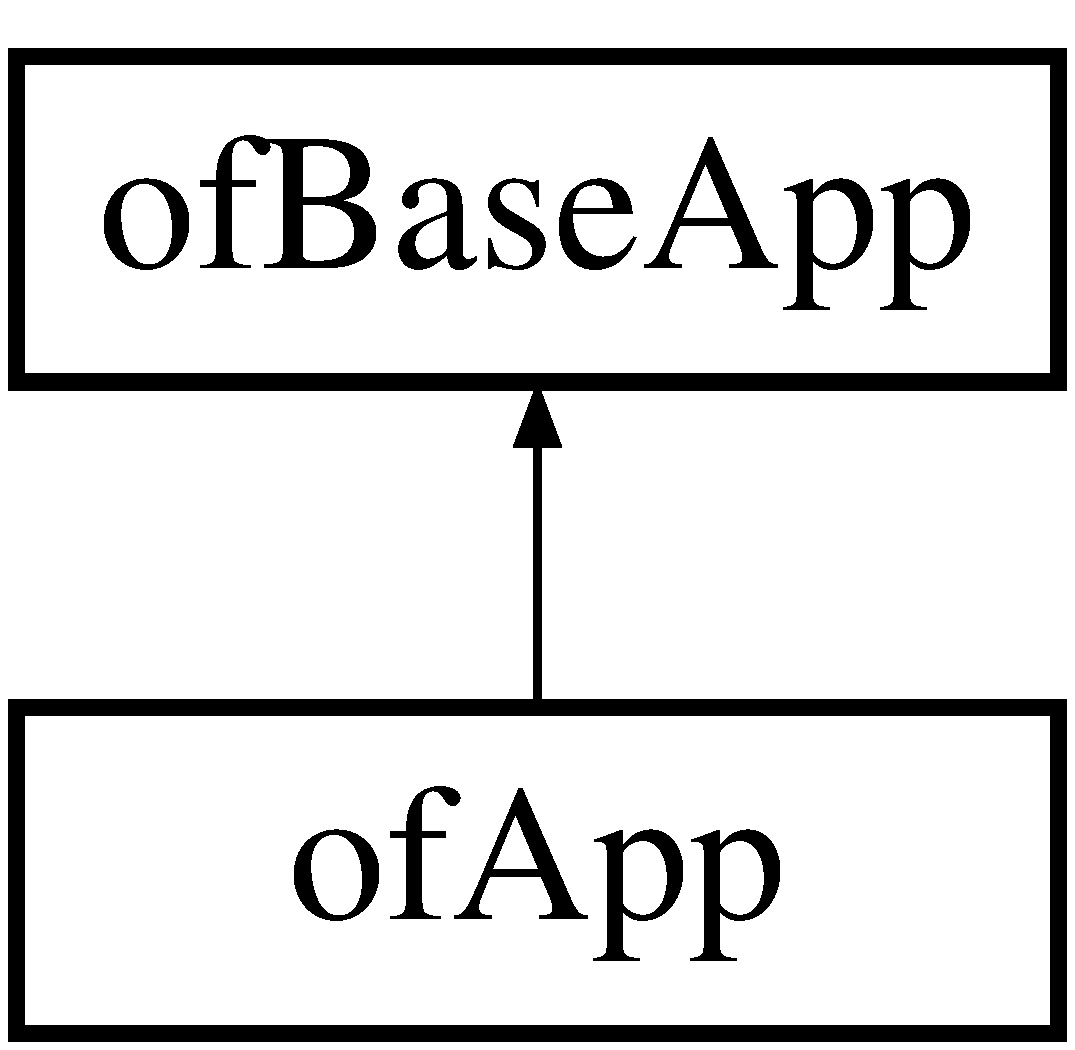
\includegraphics[height=2.000000cm]{classof_app}
\end{center}
\end{figure}
\subsection*{Public Member Functions}
\begin{DoxyCompactItemize}
\item 
\mbox{\Hypertarget{classof_app_af68eaa1366244f7a541cd08e02199c12}\label{classof_app_af68eaa1366244f7a541cd08e02199c12}} 
void {\bfseries setup} ()
\item 
\mbox{\Hypertarget{classof_app_afef41ea4aee5a22ea530afba33ae7a7b}\label{classof_app_afef41ea4aee5a22ea530afba33ae7a7b}} 
void {\bfseries update} ()
\item 
\mbox{\Hypertarget{classof_app_a75dd45437b9e317db73d8daef1ad49f8}\label{classof_app_a75dd45437b9e317db73d8daef1ad49f8}} 
void {\bfseries draw} ()
\item 
\mbox{\Hypertarget{classof_app_a957d3197364bbac8e67eaa4f15b28ad3}\label{classof_app_a957d3197364bbac8e67eaa4f15b28ad3}} 
void {\bfseries key\+Pressed} (int key)
\item 
\mbox{\Hypertarget{classof_app_aa1503a87453bcfdd395fe4acca5d91a0}\label{classof_app_aa1503a87453bcfdd395fe4acca5d91a0}} 
void {\bfseries key\+Released} (int key)
\item 
\mbox{\Hypertarget{classof_app_a158b41a606310db4633fdb817b21047c}\label{classof_app_a158b41a606310db4633fdb817b21047c}} 
void {\bfseries mouse\+Moved} (int x, int y)
\item 
\mbox{\Hypertarget{classof_app_a1ec53d1be799dc275806ff6c6548cd83}\label{classof_app_a1ec53d1be799dc275806ff6c6548cd83}} 
void {\bfseries mouse\+Dragged} (int x, int y, int button)
\item 
\mbox{\Hypertarget{classof_app_a2c2ea9c160231e55424dfd98466ef27d}\label{classof_app_a2c2ea9c160231e55424dfd98466ef27d}} 
void {\bfseries mouse\+Pressed} (int x, int y, int button)
\item 
\mbox{\Hypertarget{classof_app_aa3131f1554fc49eaa9ee0f284e48129b}\label{classof_app_aa3131f1554fc49eaa9ee0f284e48129b}} 
void {\bfseries mouse\+Released} (int x, int y, int button)
\item 
\mbox{\Hypertarget{classof_app_ae4dc1ec1513dcbe48bc78a5e4c3fac0f}\label{classof_app_ae4dc1ec1513dcbe48bc78a5e4c3fac0f}} 
void {\bfseries window\+Resized} (int w, int h)
\item 
\mbox{\Hypertarget{classof_app_aada5a79556321801567752a0e5a69bda}\label{classof_app_aada5a79556321801567752a0e5a69bda}} 
void {\bfseries drag\+Event} (of\+Drag\+Info drag\+Info)
\item 
\mbox{\Hypertarget{classof_app_a885672a72340a5e998af1d16718dc766}\label{classof_app_a885672a72340a5e998af1d16718dc766}} 
void {\bfseries got\+Message} (of\+Message msg)
\item 
\mbox{\Hypertarget{classof_app_a6ee1a7af6a715c6448f9769ff22cbabc}\label{classof_app_a6ee1a7af6a715c6448f9769ff22cbabc}} 
void {\bfseries gui\+Test001} ()
\item 
\mbox{\Hypertarget{classof_app_ad561e567741c5979497091b4ce6c1517}\label{classof_app_ad561e567741c5979497091b4ce6c1517}} 
void {\bfseries gui\+Test002} ()
\end{DoxyCompactItemize}


\subsection{Detailed Description}


The documentation for this class was generated from the following files\+:\begin{DoxyCompactItemize}
\item 
src/\+Arbutus/of\+App.\+h\item 
src/\+Arbutus/of\+App.\+cpp\end{DoxyCompactItemize}

\hypertarget{class_slider}{}\section{Slider Class Reference}
\label{class_slider}\index{Slider@{Slider}}


{\ttfamily \#include $<$Slider.\+hpp$>$}

Inheritance diagram for Slider\+:\begin{figure}[H]
\begin{center}
\leavevmode
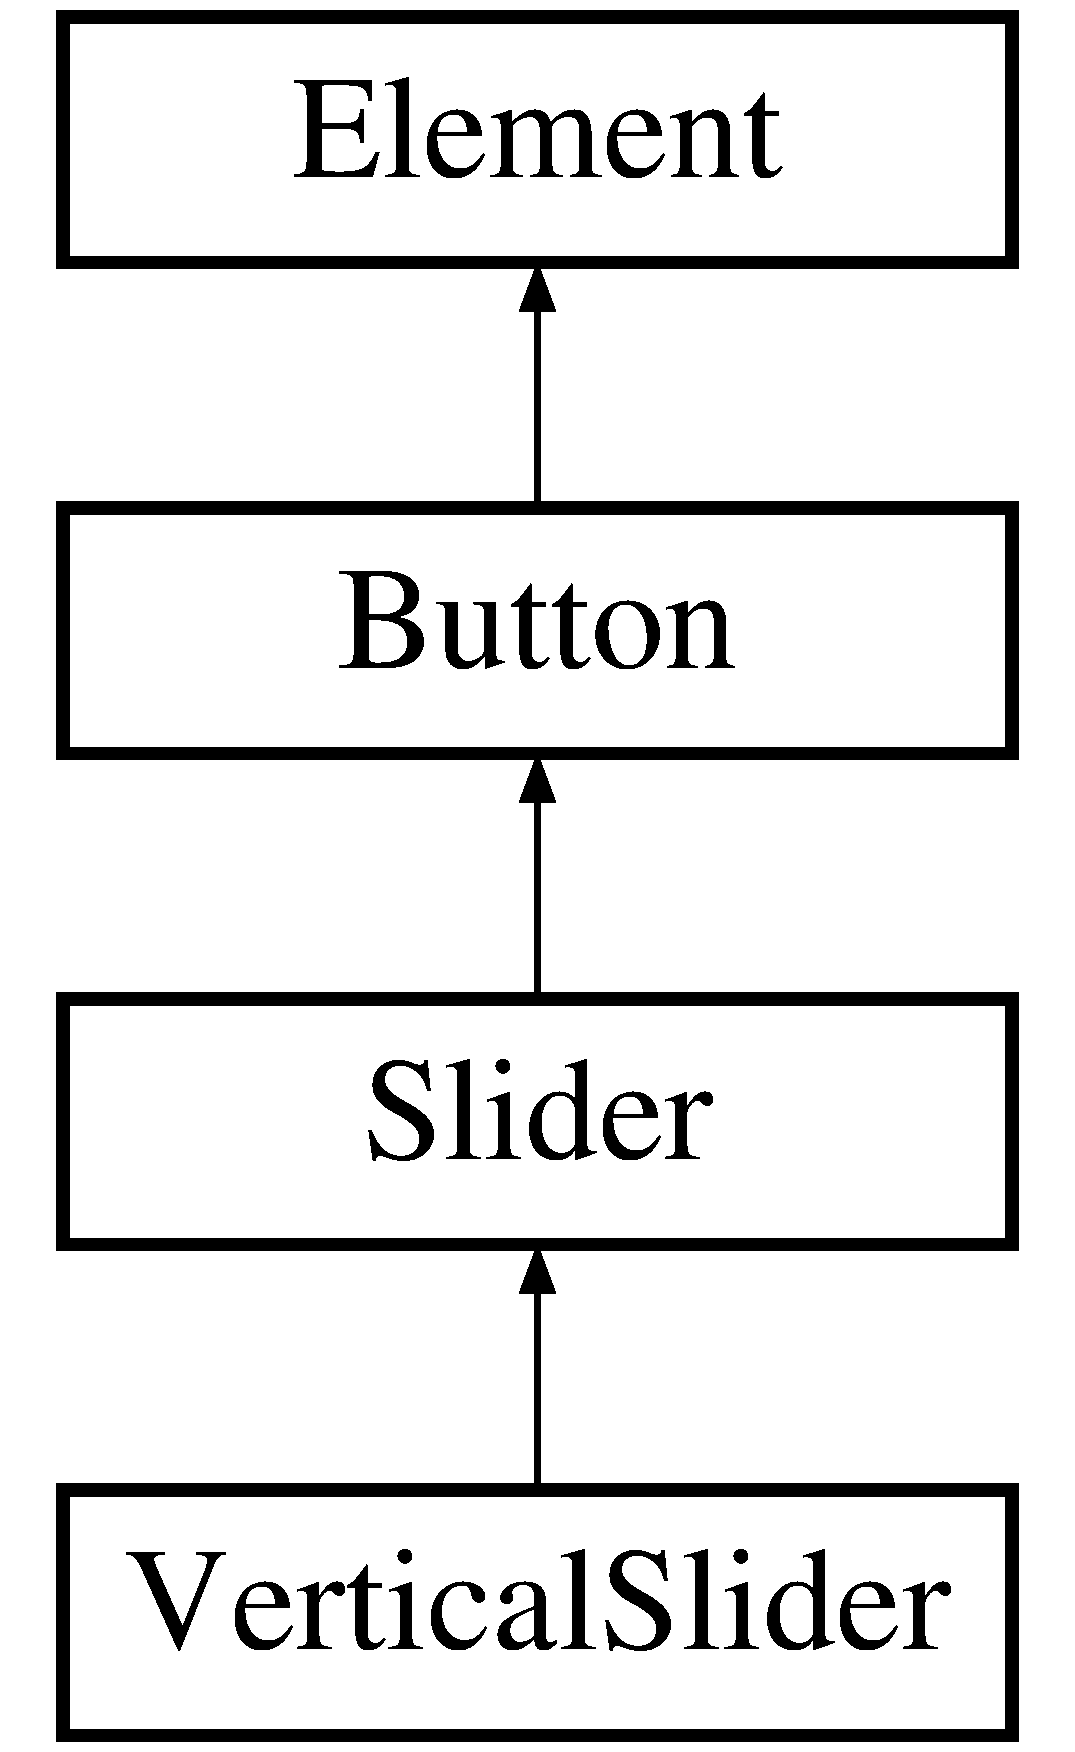
\includegraphics[height=4.000000cm]{class_slider}
\end{center}
\end{figure}
\subsection*{Public Member Functions}
\begin{DoxyCompactItemize}
\item 
\hyperlink{class_slider_a535033fada8e25ef7291d2a52e6e437b}{Slider} ()
\item 
\hyperlink{class_slider_aaca12abbe07a83f925d66339aa332028}{$\sim$\+Slider} ()
\item 
void \hyperlink{class_slider_a8bcc94829fa9c1546097da4e797665cb}{update} ()
\item 
void \hyperlink{class_slider_a1db885ef790b09aee48c7344181c5424}{draw} (N\+V\+Gcontext $\ast$vg)
\item 
of\+Color \hyperlink{class_slider_aceedad7b0b2355dd3a7923e7befcff67}{get\+Background\+Color} ()
\item 
void \hyperlink{class_slider_a834dbe16812e7bd4f0472882b0619ea9}{set} (json config)
\item 
void \hyperlink{class_slider_a2b857d6483469bde177871f38e47097e}{set\+Value} (float \+\_\+value)
\item 
float \hyperlink{class_slider_a8202efdd0e9c26277e7934949ae87537}{get\+Value} ()
\item 
void \hyperlink{class_slider_a2c072af3ce9213e5a097da49d1af8a82}{set\+On\+Change} (std\+::function$<$ void(\hyperlink{class_slider}{Slider} $\ast$slider)$>$ \+\_\+on\+Change)
\item 
virtual string \hyperlink{class_slider_a0e917883961af99856847e571a461689}{get\+Class} ()
\end{DoxyCompactItemize}
\subsection*{Protected Attributes}
\begin{DoxyCompactItemize}
\item 
\mbox{\Hypertarget{class_slider_a7e5f83db85bbc87857556df45074219c}\label{class_slider_a7e5f83db85bbc87857556df45074219c}} 
std\+::function$<$ void(\hyperlink{class_slider}{Slider} $\ast$slider)$>$ {\bfseries on\+Change} = N\+U\+LL
\item 
\mbox{\Hypertarget{class_slider_ae7a169abde25f6d0c42837b1b201f11a}\label{class_slider_ae7a169abde25f6d0c42837b1b201f11a}} 
float {\bfseries value}
\item 
\mbox{\Hypertarget{class_slider_aa9c9f7db3c8cbe8da5a7482b3b33dc24}\label{class_slider_aa9c9f7db3c8cbe8da5a7482b3b33dc24}} 
float {\bfseries max\+Value}
\item 
\mbox{\Hypertarget{class_slider_a7addbc31c8368ffd3722d3fb11abeb4d}\label{class_slider_a7addbc31c8368ffd3722d3fb11abeb4d}} 
float {\bfseries min\+Value}
\end{DoxyCompactItemize}
\subsection*{Additional Inherited Members}


\subsection{Detailed Description}
Implements a slider from the button  Descends from the button but adds new behaviour by allowing the user to drag inside and set a value. This value is between a min and a max. 

\subsection{Constructor \& Destructor Documentation}
\mbox{\Hypertarget{class_slider_a535033fada8e25ef7291d2a52e6e437b}\label{class_slider_a535033fada8e25ef7291d2a52e6e437b}} 
\index{Slider@{Slider}!Slider@{Slider}}
\index{Slider@{Slider}!Slider@{Slider}}
\subsubsection{\texorpdfstring{Slider()}{Slider()}}
{\footnotesize\ttfamily Slider\+::\+Slider (\begin{DoxyParamCaption}{ }\end{DoxyParamCaption})}

... \mbox{\Hypertarget{class_slider_aaca12abbe07a83f925d66339aa332028}\label{class_slider_aaca12abbe07a83f925d66339aa332028}} 
\index{Slider@{Slider}!````~Slider@{$\sim$\+Slider}}
\index{````~Slider@{$\sim$\+Slider}!Slider@{Slider}}
\subsubsection{\texorpdfstring{$\sim$\+Slider()}{~Slider()}}
{\footnotesize\ttfamily Slider\+::$\sim$\+Slider (\begin{DoxyParamCaption}{ }\end{DoxyParamCaption})}

... 

\subsection{Member Function Documentation}
\mbox{\Hypertarget{class_slider_a1db885ef790b09aee48c7344181c5424}\label{class_slider_a1db885ef790b09aee48c7344181c5424}} 
\index{Slider@{Slider}!draw@{draw}}
\index{draw@{draw}!Slider@{Slider}}
\subsubsection{\texorpdfstring{draw()}{draw()}}
{\footnotesize\ttfamily void Slider\+::draw (\begin{DoxyParamCaption}\item[{N\+V\+Gcontext $\ast$}]{vg }\end{DoxyParamCaption})\hspace{0.3cm}{\ttfamily [virtual]}}

... 

Reimplemented from \hyperlink{class_button_a3a6ae66dc1ebc663fc12f19ce5cb6840}{Button}.



Reimplemented in \hyperlink{class_vertical_slider_a6a5ab2800438817cc5a97c475fad9f2f}{Vertical\+Slider}.

\mbox{\Hypertarget{class_slider_aceedad7b0b2355dd3a7923e7befcff67}\label{class_slider_aceedad7b0b2355dd3a7923e7befcff67}} 
\index{Slider@{Slider}!get\+Background\+Color@{get\+Background\+Color}}
\index{get\+Background\+Color@{get\+Background\+Color}!Slider@{Slider}}
\subsubsection{\texorpdfstring{get\+Background\+Color()}{getBackgroundColor()}}
{\footnotesize\ttfamily of\+Color Slider\+::get\+Background\+Color (\begin{DoxyParamCaption}{ }\end{DoxyParamCaption})}

Calculate the background color according to the slider state \mbox{\Hypertarget{class_slider_a0e917883961af99856847e571a461689}\label{class_slider_a0e917883961af99856847e571a461689}} 
\index{Slider@{Slider}!get\+Class@{get\+Class}}
\index{get\+Class@{get\+Class}!Slider@{Slider}}
\subsubsection{\texorpdfstring{get\+Class()}{getClass()}}
{\footnotesize\ttfamily virtual string Slider\+::get\+Class (\begin{DoxyParamCaption}{ }\end{DoxyParamCaption})\hspace{0.3cm}{\ttfamily [inline]}, {\ttfamily [virtual]}}

... 

Reimplemented from \hyperlink{class_button_ad22978c530f78e58cb213436b24b37c0}{Button}.



Reimplemented in \hyperlink{class_vertical_slider_a5e13fb542bdca4cca91f96ca15b28fad}{Vertical\+Slider}.

\mbox{\Hypertarget{class_slider_a8202efdd0e9c26277e7934949ae87537}\label{class_slider_a8202efdd0e9c26277e7934949ae87537}} 
\index{Slider@{Slider}!get\+Value@{get\+Value}}
\index{get\+Value@{get\+Value}!Slider@{Slider}}
\subsubsection{\texorpdfstring{get\+Value()}{getValue()}}
{\footnotesize\ttfamily float Slider\+::get\+Value (\begin{DoxyParamCaption}{ }\end{DoxyParamCaption})}

... \mbox{\Hypertarget{class_slider_a834dbe16812e7bd4f0472882b0619ea9}\label{class_slider_a834dbe16812e7bd4f0472882b0619ea9}} 
\index{Slider@{Slider}!set@{set}}
\index{set@{set}!Slider@{Slider}}
\subsubsection{\texorpdfstring{set()}{set()}}
{\footnotesize\ttfamily void Slider\+::set (\begin{DoxyParamCaption}\item[{json}]{config }\end{DoxyParamCaption})\hspace{0.3cm}{\ttfamily [virtual]}}

... 

Reimplemented from \hyperlink{class_button_a6e7c3b800fae0b1e7765ccdafc88c28e}{Button}.



Reimplemented in \hyperlink{class_vertical_slider_a35b7771bd63647aa288f16719611b567}{Vertical\+Slider}.

\mbox{\Hypertarget{class_slider_a2c072af3ce9213e5a097da49d1af8a82}\label{class_slider_a2c072af3ce9213e5a097da49d1af8a82}} 
\index{Slider@{Slider}!set\+On\+Change@{set\+On\+Change}}
\index{set\+On\+Change@{set\+On\+Change}!Slider@{Slider}}
\subsubsection{\texorpdfstring{set\+On\+Change()}{setOnChange()}}
{\footnotesize\ttfamily void Slider\+::set\+On\+Change (\begin{DoxyParamCaption}\item[{std\+::function$<$ void(\hyperlink{class_slider}{Slider} $\ast$slider)$>$}]{\+\_\+on\+Change }\end{DoxyParamCaption})}

... \mbox{\Hypertarget{class_slider_a2b857d6483469bde177871f38e47097e}\label{class_slider_a2b857d6483469bde177871f38e47097e}} 
\index{Slider@{Slider}!set\+Value@{set\+Value}}
\index{set\+Value@{set\+Value}!Slider@{Slider}}
\subsubsection{\texorpdfstring{set\+Value()}{setValue()}}
{\footnotesize\ttfamily void Slider\+::set\+Value (\begin{DoxyParamCaption}\item[{float}]{\+\_\+value }\end{DoxyParamCaption})}

... \mbox{\Hypertarget{class_slider_a8bcc94829fa9c1546097da4e797665cb}\label{class_slider_a8bcc94829fa9c1546097da4e797665cb}} 
\index{Slider@{Slider}!update@{update}}
\index{update@{update}!Slider@{Slider}}
\subsubsection{\texorpdfstring{update()}{update()}}
{\footnotesize\ttfamily void Slider\+::update (\begin{DoxyParamCaption}{ }\end{DoxyParamCaption})\hspace{0.3cm}{\ttfamily [virtual]}}

... 

Reimplemented from \hyperlink{class_button_ad8e030c1c8846d43f3126047d4a3667f}{Button}.



Reimplemented in \hyperlink{class_vertical_slider_ae868b87e37fbdac6e4906ac6b9ad465d}{Vertical\+Slider}.



The documentation for this class was generated from the following files\+:\begin{DoxyCompactItemize}
\item 
src/\+G\+U\+I/Slider.\+hpp\item 
src/\+G\+U\+I/Slider.\+cpp\end{DoxyCompactItemize}

\hypertarget{class_splitter}{}\section{Splitter Class Reference}
\label{class_splitter}\index{Splitter@{Splitter}}


{\ttfamily \#include $<$Splitter.\+hpp$>$}

Inheritance diagram for Splitter\+:\begin{figure}[H]
\begin{center}
\leavevmode
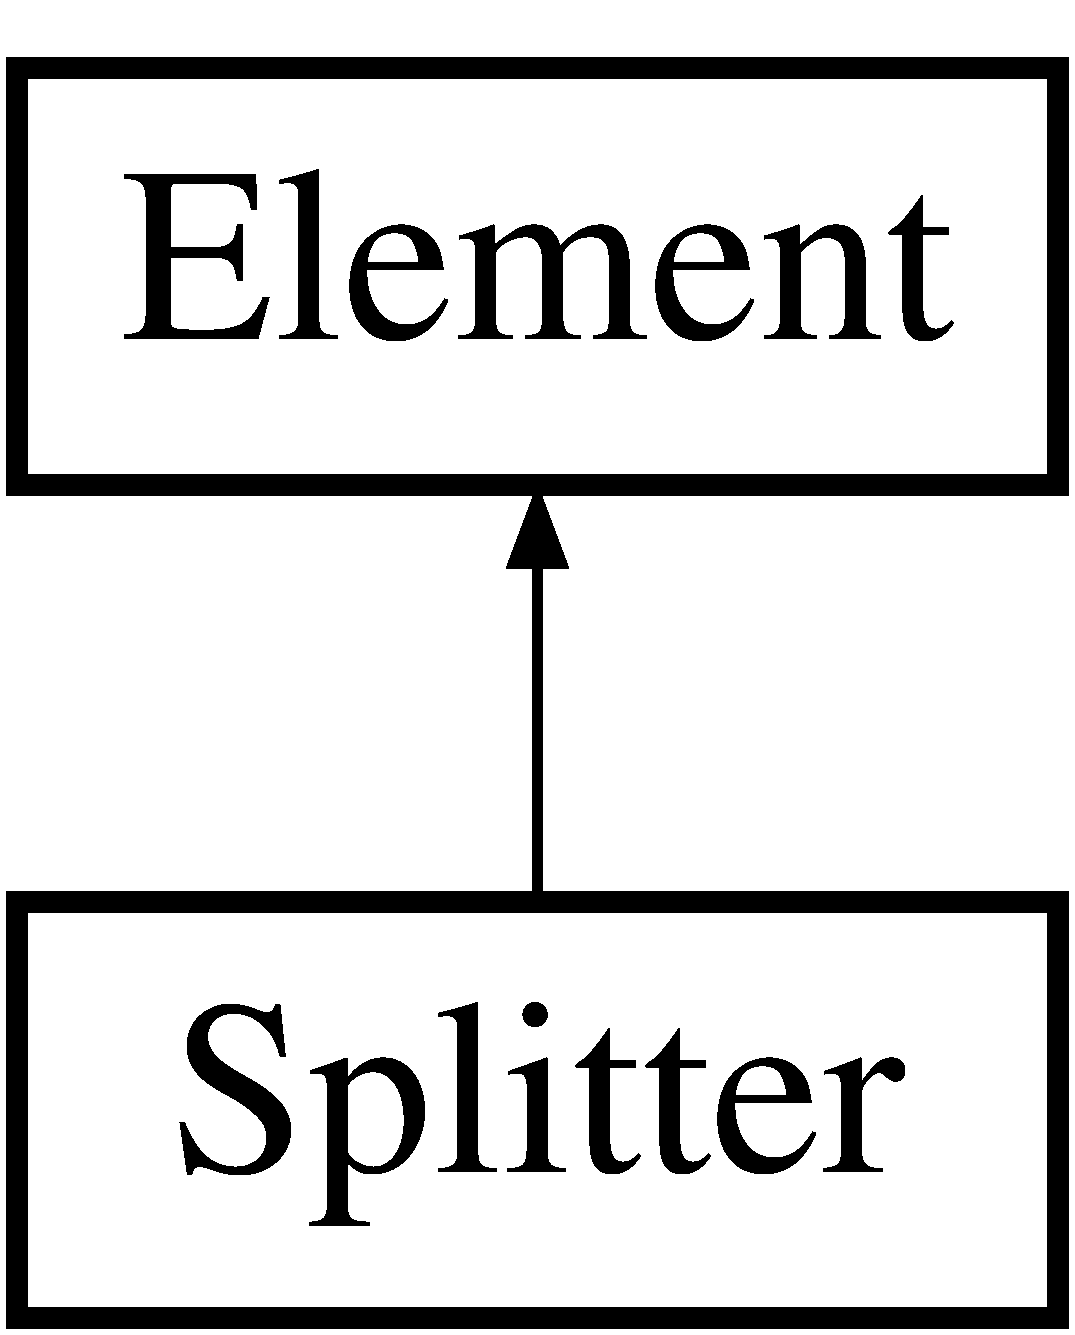
\includegraphics[height=2.000000cm]{class_splitter}
\end{center}
\end{figure}
\subsection*{Public Member Functions}
\begin{DoxyCompactItemize}
\item 
\hyperlink{class_splitter_ac62b02b8374ebe8dfdf6c34fbd59c2a1}{Splitter} ()
\item 
\hyperlink{class_splitter_a43e6a2b28ecf48a2127840a5fbf5fb3f}{$\sim$\+Splitter} ()
\item 
void \hyperlink{class_splitter_a38aab36f28b7f5b834fefae247f5c37e}{set} (json config)
\item 
void \hyperlink{class_splitter_aab6c9e9479d8208e1959eb9fbfbcdfeb}{update} ()
\item 
void \hyperlink{class_splitter_acdda30b580520e68531dfa90511a8514}{draw} (N\+V\+Gcontext $\ast$vg)
\item 
void \hyperlink{class_splitter_a4cfa6bad909de07691b290f56de1a175}{add} (\hyperlink{class_element}{Element} $\ast$element, float size)
\item 
\mbox{\Hypertarget{class_splitter_a9c611ab26d0cd4b5bdd4098ed55752fc}\label{class_splitter_a9c611ab26d0cd4b5bdd4098ed55752fc}} 
void {\bfseries calculate\+Childs\+Rects} ()
\end{DoxyCompactItemize}
\subsection*{Protected Member Functions}
\begin{DoxyCompactItemize}
\item 
\mbox{\Hypertarget{class_splitter_a9f1eec80a14195e074e93e0d4305d2f0}\label{class_splitter_a9f1eec80a14195e074e93e0d4305d2f0}} 
void {\bfseries calculate\+Rect} ()
\end{DoxyCompactItemize}
\subsection*{Protected Attributes}
\begin{DoxyCompactItemize}
\item 
\mbox{\Hypertarget{class_splitter_a80d42af90ddecf61e0bd988fa0abc877}\label{class_splitter_a80d42af90ddecf61e0bd988fa0abc877}} 
Splitter\+Type {\bfseries type}
\item 
\mbox{\Hypertarget{class_splitter_a1fe850cd6ee1699cc00ca16b2b2a2992}\label{class_splitter_a1fe850cd6ee1699cc00ca16b2b2a2992}} 
std\+::vector$<$ \hyperlink{struct_splitter_child}{Splitter\+Child} $>$ {\bfseries childs}
\end{DoxyCompactItemize}
\subsection*{Additional Inherited Members}


\subsection{Detailed Description}
Divides the area of the parent into several elements  Takes the entire area of the parent or the whole screen of no parent. Divides it into the given number of requested zones. each zone needs to define a percentage (float values 0 to 1). the total percentage must be 1. 

\subsection{Constructor \& Destructor Documentation}
\mbox{\Hypertarget{class_splitter_ac62b02b8374ebe8dfdf6c34fbd59c2a1}\label{class_splitter_ac62b02b8374ebe8dfdf6c34fbd59c2a1}} 
\index{Splitter@{Splitter}!Splitter@{Splitter}}
\index{Splitter@{Splitter}!Splitter@{Splitter}}
\subsubsection{\texorpdfstring{Splitter()}{Splitter()}}
{\footnotesize\ttfamily Splitter\+::\+Splitter (\begin{DoxyParamCaption}{ }\end{DoxyParamCaption})}

... \mbox{\Hypertarget{class_splitter_a43e6a2b28ecf48a2127840a5fbf5fb3f}\label{class_splitter_a43e6a2b28ecf48a2127840a5fbf5fb3f}} 
\index{Splitter@{Splitter}!````~Splitter@{$\sim$\+Splitter}}
\index{````~Splitter@{$\sim$\+Splitter}!Splitter@{Splitter}}
\subsubsection{\texorpdfstring{$\sim$\+Splitter()}{~Splitter()}}
{\footnotesize\ttfamily Splitter\+::$\sim$\+Splitter (\begin{DoxyParamCaption}{ }\end{DoxyParamCaption})}

... 

\subsection{Member Function Documentation}
\mbox{\Hypertarget{class_splitter_a4cfa6bad909de07691b290f56de1a175}\label{class_splitter_a4cfa6bad909de07691b290f56de1a175}} 
\index{Splitter@{Splitter}!add@{add}}
\index{add@{add}!Splitter@{Splitter}}
\subsubsection{\texorpdfstring{add()}{add()}}
{\footnotesize\ttfamily void Splitter\+::add (\begin{DoxyParamCaption}\item[{\hyperlink{class_element}{Element} $\ast$}]{element,  }\item[{float}]{size }\end{DoxyParamCaption})}

Adds a new element to the splitter at the end \mbox{\Hypertarget{class_splitter_acdda30b580520e68531dfa90511a8514}\label{class_splitter_acdda30b580520e68531dfa90511a8514}} 
\index{Splitter@{Splitter}!draw@{draw}}
\index{draw@{draw}!Splitter@{Splitter}}
\subsubsection{\texorpdfstring{draw()}{draw()}}
{\footnotesize\ttfamily void Splitter\+::draw (\begin{DoxyParamCaption}\item[{N\+V\+Gcontext $\ast$}]{vg }\end{DoxyParamCaption})\hspace{0.3cm}{\ttfamily [virtual]}}

... 

Reimplemented from \hyperlink{class_element_a37c9abed5bec87d9ce0a5e74fb872f34}{Element}.

\mbox{\Hypertarget{class_splitter_a38aab36f28b7f5b834fefae247f5c37e}\label{class_splitter_a38aab36f28b7f5b834fefae247f5c37e}} 
\index{Splitter@{Splitter}!set@{set}}
\index{set@{set}!Splitter@{Splitter}}
\subsubsection{\texorpdfstring{set()}{set()}}
{\footnotesize\ttfamily void Splitter\+::set (\begin{DoxyParamCaption}\item[{json}]{config }\end{DoxyParamCaption})\hspace{0.3cm}{\ttfamily [virtual]}}

... 

Reimplemented from \hyperlink{class_element_af89dcf0a470753cf1fecd8556a802c63}{Element}.

\mbox{\Hypertarget{class_splitter_aab6c9e9479d8208e1959eb9fbfbcdfeb}\label{class_splitter_aab6c9e9479d8208e1959eb9fbfbcdfeb}} 
\index{Splitter@{Splitter}!update@{update}}
\index{update@{update}!Splitter@{Splitter}}
\subsubsection{\texorpdfstring{update()}{update()}}
{\footnotesize\ttfamily void Splitter\+::update (\begin{DoxyParamCaption}{ }\end{DoxyParamCaption})\hspace{0.3cm}{\ttfamily [virtual]}}

... 

Reimplemented from \hyperlink{class_element_a35de04f6ab79440bb44083d8b300b87d}{Element}.



The documentation for this class was generated from the following files\+:\begin{DoxyCompactItemize}
\item 
src/\+G\+U\+I/Splitter.\+hpp\item 
src/\+G\+U\+I/Splitter.\+cpp\end{DoxyCompactItemize}

\hypertarget{struct_splitter_child}{}\section{Splitter\+Child Struct Reference}
\label{struct_splitter_child}\index{Splitter\+Child@{Splitter\+Child}}
\subsection*{Public Attributes}
\begin{DoxyCompactItemize}
\item 
\mbox{\Hypertarget{struct_splitter_child_aca1e3e626b40621df7cbf4eb084fd82d}\label{struct_splitter_child_aca1e3e626b40621df7cbf4eb084fd82d}} 
\hyperlink{class_element}{Element} $\ast$ {\bfseries element}
\item 
\mbox{\Hypertarget{struct_splitter_child_a4d6ca3e1ca70ed7e931990bc95161c66}\label{struct_splitter_child_a4d6ca3e1ca70ed7e931990bc95161c66}} 
float {\bfseries size}
\end{DoxyCompactItemize}


The documentation for this struct was generated from the following file\+:\begin{DoxyCompactItemize}
\item 
src/\+G\+U\+I/Splitter.\+hpp\end{DoxyCompactItemize}

\hypertarget{class_trigger_visual_action}{}\section{Trigger\+Visual\+Action Class Reference}
\label{class_trigger_visual_action}\index{Trigger\+Visual\+Action@{Trigger\+Visual\+Action}}


{\ttfamily \#include $<$G\+U\+I\+Style.\+hpp$>$}



\subsection{Detailed Description}


The documentation for this class was generated from the following file\+:\begin{DoxyCompactItemize}
\item 
src/\+G\+U\+I/G\+U\+I\+Style.\+hpp\end{DoxyCompactItemize}

\hypertarget{class_vertical_slider}{}\section{Vertical\+Slider Class Reference}
\label{class_vertical_slider}\index{Vertical\+Slider@{Vertical\+Slider}}


{\ttfamily \#include $<$Vertical\+Slider.\+hpp$>$}

Inheritance diagram for Vertical\+Slider\+:\begin{figure}[H]
\begin{center}
\leavevmode
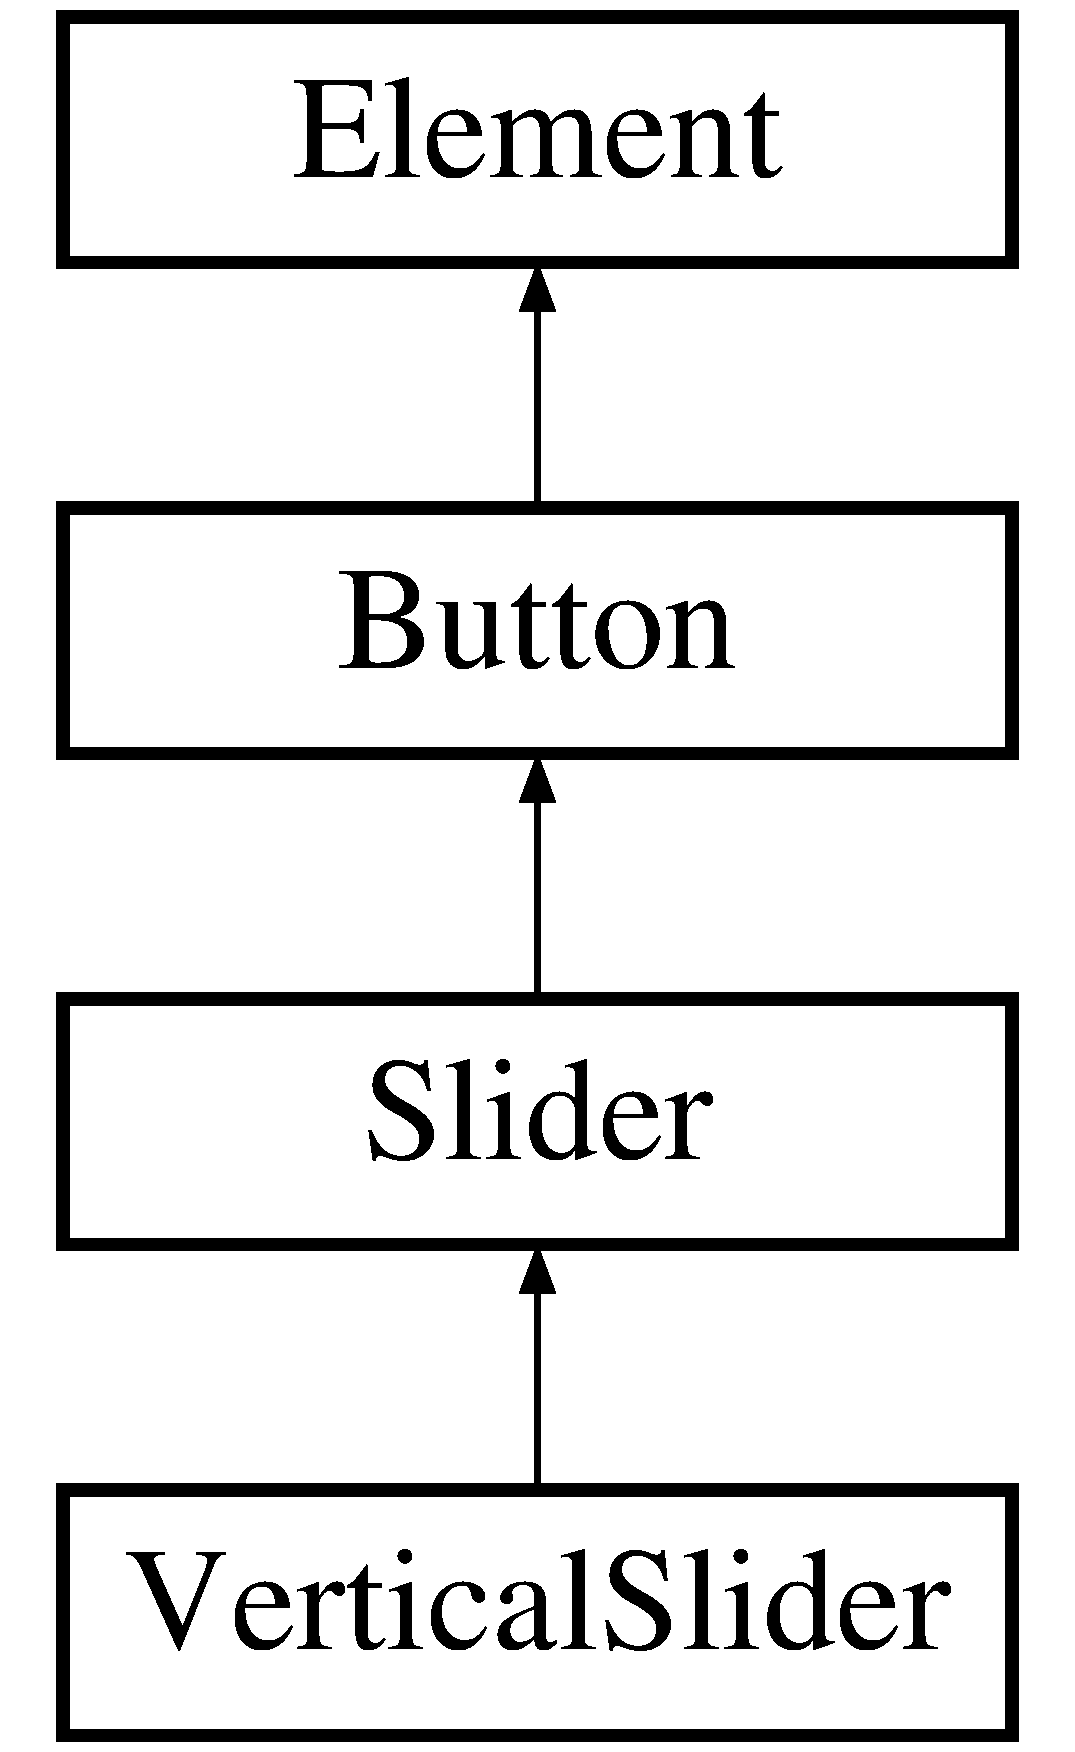
\includegraphics[height=4.000000cm]{class_vertical_slider}
\end{center}
\end{figure}
\subsection*{Public Member Functions}
\begin{DoxyCompactItemize}
\item 
\hyperlink{class_vertical_slider_af83ca315bf665ac96d29df5c4e32ecc0}{Vertical\+Slider} ()
\item 
\hyperlink{class_vertical_slider_ace98a29d39b256e37628334c2cc69822}{$\sim$\+Vertical\+Slider} ()
\item 
void \hyperlink{class_vertical_slider_ae868b87e37fbdac6e4906ac6b9ad465d}{update} ()
\item 
void \hyperlink{class_vertical_slider_a6a5ab2800438817cc5a97c475fad9f2f}{draw} (N\+V\+Gcontext $\ast$vg)
\item 
void \hyperlink{class_vertical_slider_a35b7771bd63647aa288f16719611b567}{set} (json config)
\item 
virtual string \hyperlink{class_vertical_slider_a5e13fb542bdca4cca91f96ca15b28fad}{get\+Class} ()
\end{DoxyCompactItemize}
\subsection*{Additional Inherited Members}


\subsection{Detailed Description}
A vertical oriented slider without caption (only because I haven\textquotesingle{}t figured out how to rotate the text. this should be changed soon!)  

\subsection{Constructor \& Destructor Documentation}
\mbox{\Hypertarget{class_vertical_slider_af83ca315bf665ac96d29df5c4e32ecc0}\label{class_vertical_slider_af83ca315bf665ac96d29df5c4e32ecc0}} 
\index{Vertical\+Slider@{Vertical\+Slider}!Vertical\+Slider@{Vertical\+Slider}}
\index{Vertical\+Slider@{Vertical\+Slider}!Vertical\+Slider@{Vertical\+Slider}}
\subsubsection{\texorpdfstring{Vertical\+Slider()}{VerticalSlider()}}
{\footnotesize\ttfamily Vertical\+Slider\+::\+Vertical\+Slider (\begin{DoxyParamCaption}{ }\end{DoxyParamCaption})}

... \mbox{\Hypertarget{class_vertical_slider_ace98a29d39b256e37628334c2cc69822}\label{class_vertical_slider_ace98a29d39b256e37628334c2cc69822}} 
\index{Vertical\+Slider@{Vertical\+Slider}!````~Vertical\+Slider@{$\sim$\+Vertical\+Slider}}
\index{````~Vertical\+Slider@{$\sim$\+Vertical\+Slider}!Vertical\+Slider@{Vertical\+Slider}}
\subsubsection{\texorpdfstring{$\sim$\+Vertical\+Slider()}{~VerticalSlider()}}
{\footnotesize\ttfamily Vertical\+Slider\+::$\sim$\+Vertical\+Slider (\begin{DoxyParamCaption}{ }\end{DoxyParamCaption})}

... 

\subsection{Member Function Documentation}
\mbox{\Hypertarget{class_vertical_slider_a6a5ab2800438817cc5a97c475fad9f2f}\label{class_vertical_slider_a6a5ab2800438817cc5a97c475fad9f2f}} 
\index{Vertical\+Slider@{Vertical\+Slider}!draw@{draw}}
\index{draw@{draw}!Vertical\+Slider@{Vertical\+Slider}}
\subsubsection{\texorpdfstring{draw()}{draw()}}
{\footnotesize\ttfamily void Vertical\+Slider\+::draw (\begin{DoxyParamCaption}\item[{N\+V\+Gcontext $\ast$}]{vg }\end{DoxyParamCaption})\hspace{0.3cm}{\ttfamily [virtual]}}

... 

Reimplemented from \hyperlink{class_slider_a1db885ef790b09aee48c7344181c5424}{Slider}.

\mbox{\Hypertarget{class_vertical_slider_a5e13fb542bdca4cca91f96ca15b28fad}\label{class_vertical_slider_a5e13fb542bdca4cca91f96ca15b28fad}} 
\index{Vertical\+Slider@{Vertical\+Slider}!get\+Class@{get\+Class}}
\index{get\+Class@{get\+Class}!Vertical\+Slider@{Vertical\+Slider}}
\subsubsection{\texorpdfstring{get\+Class()}{getClass()}}
{\footnotesize\ttfamily virtual string Vertical\+Slider\+::get\+Class (\begin{DoxyParamCaption}{ }\end{DoxyParamCaption})\hspace{0.3cm}{\ttfamily [inline]}, {\ttfamily [virtual]}}

... 

Reimplemented from \hyperlink{class_slider_a0e917883961af99856847e571a461689}{Slider}.

\mbox{\Hypertarget{class_vertical_slider_a35b7771bd63647aa288f16719611b567}\label{class_vertical_slider_a35b7771bd63647aa288f16719611b567}} 
\index{Vertical\+Slider@{Vertical\+Slider}!set@{set}}
\index{set@{set}!Vertical\+Slider@{Vertical\+Slider}}
\subsubsection{\texorpdfstring{set()}{set()}}
{\footnotesize\ttfamily void Vertical\+Slider\+::set (\begin{DoxyParamCaption}\item[{json}]{config }\end{DoxyParamCaption})\hspace{0.3cm}{\ttfamily [virtual]}}

... 

Reimplemented from \hyperlink{class_slider_a834dbe16812e7bd4f0472882b0619ea9}{Slider}.

\mbox{\Hypertarget{class_vertical_slider_ae868b87e37fbdac6e4906ac6b9ad465d}\label{class_vertical_slider_ae868b87e37fbdac6e4906ac6b9ad465d}} 
\index{Vertical\+Slider@{Vertical\+Slider}!update@{update}}
\index{update@{update}!Vertical\+Slider@{Vertical\+Slider}}
\subsubsection{\texorpdfstring{update()}{update()}}
{\footnotesize\ttfamily void Vertical\+Slider\+::update (\begin{DoxyParamCaption}{ }\end{DoxyParamCaption})\hspace{0.3cm}{\ttfamily [virtual]}}

... 

Reimplemented from \hyperlink{class_slider_a8bcc94829fa9c1546097da4e797665cb}{Slider}.



The documentation for this class was generated from the following files\+:\begin{DoxyCompactItemize}
\item 
src/\+G\+U\+I/Vertical\+Slider.\+hpp\item 
src/\+G\+U\+I/Vertical\+Slider.\+cpp\end{DoxyCompactItemize}

\hypertarget{class_viewport}{}\section{Viewport Class Reference}
\label{class_viewport}\index{Viewport@{Viewport}}


{\ttfamily \#include $<$Viewport.\+hpp$>$}

Inheritance diagram for Viewport\+:\begin{figure}[H]
\begin{center}
\leavevmode
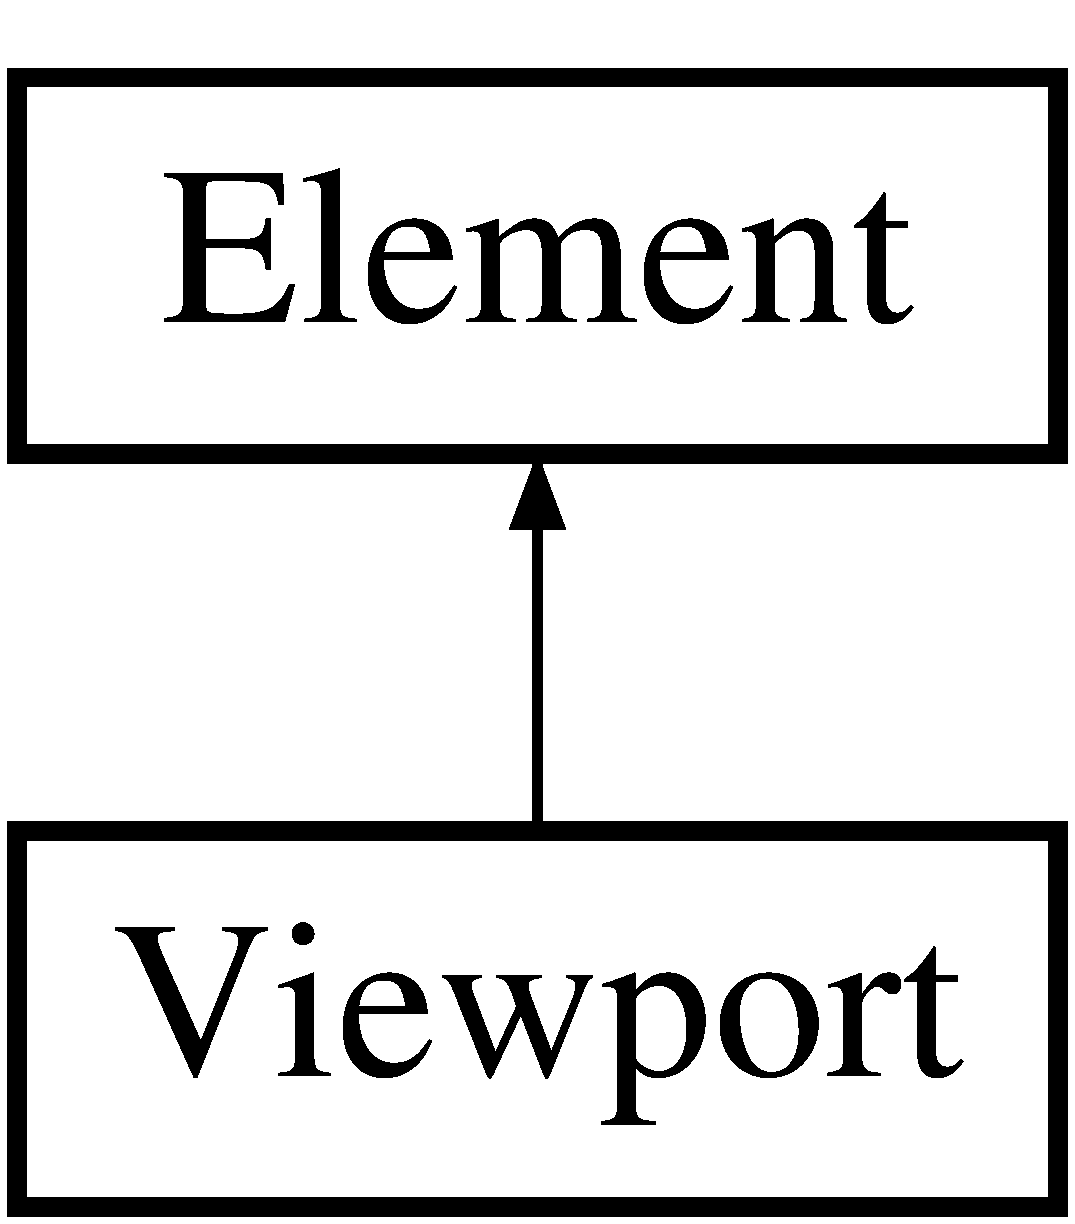
\includegraphics[height=2.000000cm]{class_viewport}
\end{center}
\end{figure}
\subsection*{Public Member Functions}
\begin{DoxyCompactItemize}
\item 
\hyperlink{class_viewport_a9fde8f966d9802dd42254acf0ed05386}{Viewport} ()
\item 
\hyperlink{class_viewport_a1e18a1ff4a52be33ef63d25034561850}{$\sim$\+Viewport} ()
\item 
void \hyperlink{class_viewport_a96703fae50a7a103da0a576c55fbdea5}{set} (json config)
\item 
virtual void \hyperlink{class_viewport_a7997e0e684a4f8b5709f4d98be6cebb4}{update} ()
\item 
virtual void \hyperlink{class_viewport_a89204037b4982e95495ffb239e9974fc}{draw} (N\+V\+Gcontext $\ast$vg)
\item 
virtual string \hyperlink{class_viewport_adef77198ff36001558b7a29247cedc90}{get\+Class} ()
\item 
of\+Rectangle \hyperlink{class_viewport_a2b7530dfc9d4df664f3874c8ec17d86e}{calculate\+Drawing\+Rect\+For\+Element} (\hyperlink{class_element}{Element} $\ast$element)
\item 
void \hyperlink{class_viewport_a48a9793ff0b244d0618355a32176c459}{set\+Scroll\+PositionY} (float position)
\item 
void \hyperlink{class_viewport_a6343db7258b534ee48e144f94af35e6e}{set\+Scroll\+PositionX} (float position)
\item 
\hyperlink{class_element}{Element} $\ast$ \hyperlink{class_viewport_a91661e99e68106bb29cf20807c5a167c}{add} (\hyperlink{class_element}{Element} $\ast$new\+Element)
\item 
void \hyperlink{class_viewport_a7c8543f8de21b83de2d850c3597d40ec}{resize} (of\+Rectangle new\+Rect)
\end{DoxyCompactItemize}
\subsection*{Protected Attributes}
\begin{DoxyCompactItemize}
\item 
\mbox{\Hypertarget{class_viewport_a771c72174c19e72d2988d8203bb0bf70}\label{class_viewport_a771c72174c19e72d2988d8203bb0bf70}} 
\hyperlink{class_element}{Element} $\ast$ {\bfseries component}
\item 
\mbox{\Hypertarget{class_viewport_a23c68fffb90641759e39f0a6eddfcca8}\label{class_viewport_a23c68fffb90641759e39f0a6eddfcca8}} 
float {\bfseries overflowX}
\item 
\mbox{\Hypertarget{class_viewport_a13662e1986bf472dc8150bfd82193034}\label{class_viewport_a13662e1986bf472dc8150bfd82193034}} 
float {\bfseries overflowY}
\item 
\mbox{\Hypertarget{class_viewport_a1b3a096a9c0812c85665bf1991d4e5e1}\label{class_viewport_a1b3a096a9c0812c85665bf1991d4e5e1}} 
float {\bfseries scroll\+PositionX}
\item 
\mbox{\Hypertarget{class_viewport_a0dd61a3009e40e8979110d8075f1962c}\label{class_viewport_a0dd61a3009e40e8979110d8075f1962c}} 
float {\bfseries scroll\+PositionY}
\item 
\mbox{\Hypertarget{class_viewport_ae3d3b8f45b685d9565e5ae4efe70e7dd}\label{class_viewport_ae3d3b8f45b685d9565e5ae4efe70e7dd}} 
float {\bfseries total\+Height}
\item 
\mbox{\Hypertarget{class_viewport_a111086588062bf7b9097a38bcf0d22d3}\label{class_viewport_a111086588062bf7b9097a38bcf0d22d3}} 
float {\bfseries total\+Width}
\end{DoxyCompactItemize}
\subsection*{Additional Inherited Members}


\subsection{Detailed Description}
Implements a scrollable area that can contain elements. The \hyperlink{class_element}{Element} class already allows this but isn\textquotesingle{}t scrollable.  

\subsection{Constructor \& Destructor Documentation}
\mbox{\Hypertarget{class_viewport_a9fde8f966d9802dd42254acf0ed05386}\label{class_viewport_a9fde8f966d9802dd42254acf0ed05386}} 
\index{Viewport@{Viewport}!Viewport@{Viewport}}
\index{Viewport@{Viewport}!Viewport@{Viewport}}
\subsubsection{\texorpdfstring{Viewport()}{Viewport()}}
{\footnotesize\ttfamily Viewport\+::\+Viewport (\begin{DoxyParamCaption}{ }\end{DoxyParamCaption})}

... \mbox{\Hypertarget{class_viewport_a1e18a1ff4a52be33ef63d25034561850}\label{class_viewport_a1e18a1ff4a52be33ef63d25034561850}} 
\index{Viewport@{Viewport}!````~Viewport@{$\sim$\+Viewport}}
\index{````~Viewport@{$\sim$\+Viewport}!Viewport@{Viewport}}
\subsubsection{\texorpdfstring{$\sim$\+Viewport()}{~Viewport()}}
{\footnotesize\ttfamily Viewport\+::$\sim$\+Viewport (\begin{DoxyParamCaption}{ }\end{DoxyParamCaption})}

... 

\subsection{Member Function Documentation}
\mbox{\Hypertarget{class_viewport_a91661e99e68106bb29cf20807c5a167c}\label{class_viewport_a91661e99e68106bb29cf20807c5a167c}} 
\index{Viewport@{Viewport}!add@{add}}
\index{add@{add}!Viewport@{Viewport}}
\subsubsection{\texorpdfstring{add()}{add()}}
{\footnotesize\ttfamily \hyperlink{class_element}{Element} $\ast$ Viewport\+::add (\begin{DoxyParamCaption}\item[{\hyperlink{class_element}{Element} $\ast$}]{new\+Element }\end{DoxyParamCaption})}

Add a new element to the viewport \mbox{\Hypertarget{class_viewport_a2b7530dfc9d4df664f3874c8ec17d86e}\label{class_viewport_a2b7530dfc9d4df664f3874c8ec17d86e}} 
\index{Viewport@{Viewport}!calculate\+Drawing\+Rect\+For\+Element@{calculate\+Drawing\+Rect\+For\+Element}}
\index{calculate\+Drawing\+Rect\+For\+Element@{calculate\+Drawing\+Rect\+For\+Element}!Viewport@{Viewport}}
\subsubsection{\texorpdfstring{calculate\+Drawing\+Rect\+For\+Element()}{calculateDrawingRectForElement()}}
{\footnotesize\ttfamily of\+Rectangle Viewport\+::calculate\+Drawing\+Rect\+For\+Element (\begin{DoxyParamCaption}\item[{\hyperlink{class_element}{Element} $\ast$}]{element }\end{DoxyParamCaption})}

... \mbox{\Hypertarget{class_viewport_a89204037b4982e95495ffb239e9974fc}\label{class_viewport_a89204037b4982e95495ffb239e9974fc}} 
\index{Viewport@{Viewport}!draw@{draw}}
\index{draw@{draw}!Viewport@{Viewport}}
\subsubsection{\texorpdfstring{draw()}{draw()}}
{\footnotesize\ttfamily void Viewport\+::draw (\begin{DoxyParamCaption}\item[{N\+V\+Gcontext $\ast$}]{vg }\end{DoxyParamCaption})\hspace{0.3cm}{\ttfamily [virtual]}}

... 

Reimplemented from \hyperlink{class_element_a37c9abed5bec87d9ce0a5e74fb872f34}{Element}.

\mbox{\Hypertarget{class_viewport_adef77198ff36001558b7a29247cedc90}\label{class_viewport_adef77198ff36001558b7a29247cedc90}} 
\index{Viewport@{Viewport}!get\+Class@{get\+Class}}
\index{get\+Class@{get\+Class}!Viewport@{Viewport}}
\subsubsection{\texorpdfstring{get\+Class()}{getClass()}}
{\footnotesize\ttfamily virtual string Viewport\+::get\+Class (\begin{DoxyParamCaption}{ }\end{DoxyParamCaption})\hspace{0.3cm}{\ttfamily [inline]}, {\ttfamily [virtual]}}

... 

Reimplemented from \hyperlink{class_element}{Element}.

\mbox{\Hypertarget{class_viewport_a7c8543f8de21b83de2d850c3597d40ec}\label{class_viewport_a7c8543f8de21b83de2d850c3597d40ec}} 
\index{Viewport@{Viewport}!resize@{resize}}
\index{resize@{resize}!Viewport@{Viewport}}
\subsubsection{\texorpdfstring{resize()}{resize()}}
{\footnotesize\ttfamily void Viewport\+::resize (\begin{DoxyParamCaption}\item[{of\+Rectangle}]{new\+Rect }\end{DoxyParamCaption})\hspace{0.3cm}{\ttfamily [virtual]}}

Sets the new rect 

Reimplemented from \hyperlink{class_element_a9d78e1489e80f210a8f5cc9e5d5b07d3}{Element}.

\mbox{\Hypertarget{class_viewport_a96703fae50a7a103da0a576c55fbdea5}\label{class_viewport_a96703fae50a7a103da0a576c55fbdea5}} 
\index{Viewport@{Viewport}!set@{set}}
\index{set@{set}!Viewport@{Viewport}}
\subsubsection{\texorpdfstring{set()}{set()}}
{\footnotesize\ttfamily void Viewport\+::set (\begin{DoxyParamCaption}\item[{json}]{config }\end{DoxyParamCaption})\hspace{0.3cm}{\ttfamily [virtual]}}

... 

Reimplemented from \hyperlink{class_element_af89dcf0a470753cf1fecd8556a802c63}{Element}.

\mbox{\Hypertarget{class_viewport_a6343db7258b534ee48e144f94af35e6e}\label{class_viewport_a6343db7258b534ee48e144f94af35e6e}} 
\index{Viewport@{Viewport}!set\+Scroll\+PositionX@{set\+Scroll\+PositionX}}
\index{set\+Scroll\+PositionX@{set\+Scroll\+PositionX}!Viewport@{Viewport}}
\subsubsection{\texorpdfstring{set\+Scroll\+Position\+X()}{setScrollPositionX()}}
{\footnotesize\ttfamily void Viewport\+::set\+Scroll\+PositionX (\begin{DoxyParamCaption}\item[{float}]{position }\end{DoxyParamCaption})}

... \mbox{\Hypertarget{class_viewport_a48a9793ff0b244d0618355a32176c459}\label{class_viewport_a48a9793ff0b244d0618355a32176c459}} 
\index{Viewport@{Viewport}!set\+Scroll\+PositionY@{set\+Scroll\+PositionY}}
\index{set\+Scroll\+PositionY@{set\+Scroll\+PositionY}!Viewport@{Viewport}}
\subsubsection{\texorpdfstring{set\+Scroll\+Position\+Y()}{setScrollPositionY()}}
{\footnotesize\ttfamily void Viewport\+::set\+Scroll\+PositionY (\begin{DoxyParamCaption}\item[{float}]{position }\end{DoxyParamCaption})}

... \mbox{\Hypertarget{class_viewport_a7997e0e684a4f8b5709f4d98be6cebb4}\label{class_viewport_a7997e0e684a4f8b5709f4d98be6cebb4}} 
\index{Viewport@{Viewport}!update@{update}}
\index{update@{update}!Viewport@{Viewport}}
\subsubsection{\texorpdfstring{update()}{update()}}
{\footnotesize\ttfamily void Viewport\+::update (\begin{DoxyParamCaption}{ }\end{DoxyParamCaption})\hspace{0.3cm}{\ttfamily [virtual]}}

... 

Reimplemented from \hyperlink{class_element_a35de04f6ab79440bb44083d8b300b87d}{Element}.



The documentation for this class was generated from the following files\+:\begin{DoxyCompactItemize}
\item 
src/\+G\+U\+I/Viewport.\+hpp\item 
src/\+G\+U\+I/Viewport.\+cpp\end{DoxyCompactItemize}

%--- End generated contents ---

% Index
\backmatter
\newpage
\phantomsection
\clearemptydoublepage
\addcontentsline{toc}{chapter}{Index}
\printindex

\end{document}
